%Made By Thomas Debelle fuck Thomas
\documentclass{report}
\usepackage[a4paper, total={6in, 9in}]{geometry}
\usepackage[utf8]{inputenc}
\usepackage[french]{babel}
\usepackage{graphicx}
\usepackage{graphics}
\usepackage{colortbl}
\usepackage[T1]{fontenc}
\usepackage{amsmath}
\usepackage{hyperref}
\usepackage{array}
\usepackage{amssymb}
\usepackage{colortbl}
\usepackage{color}
\usepackage{listings}
\usepackage{xcolor}
\usepackage{array}
\usepackage{float}
\usepackage{amsfonts}
\usepackage{tikz}
\usepackage{fancyhdr}
\usepackage{titlesec}
\usepackage{xparse}
\usepackage{wrapfig}

\hypersetup{
    colorlinks=true,
    linkcolor=black,
    filecolor=magenta,
    urlcolor=cyan,
    pdftitle={Overleaf Example},
    pdfpagemode=FullScreen,
    }
\begin{document}


\begin{titlepage}
    \begin{figure}
        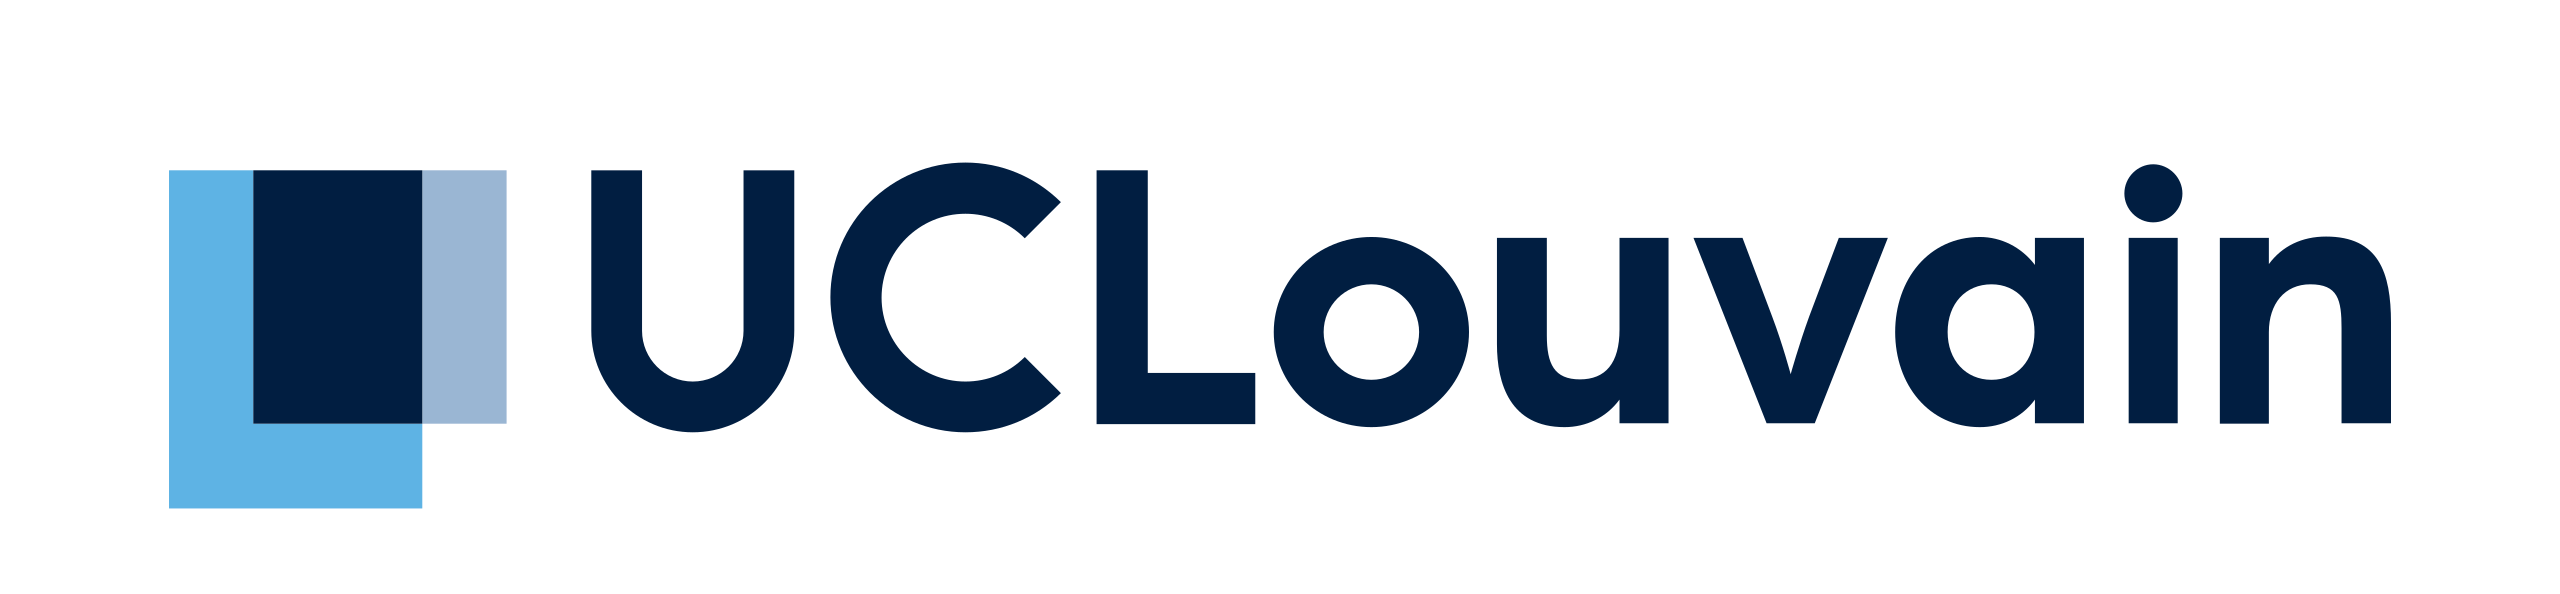
\includegraphics[height = 2cm]{UCL_Logo.png}
        \label{fig:my_label}
    \end{figure}

    \hspace*{100cm}
    \centering
    \vspace*{7cm}

    {\Huge \textbf{Résumé de LEPL1106}}\\
    \vspace*{0.25cm}
    compilation du \today\\
    \vspace*{0.25cm}
    \Large{Thomas Debelle}\\

    \vspace*{9.5cm}
    {\Large Juin 2023}
\end{titlepage}


\tableofcontents
\newpage

\section*{Préface}

Bonjour à toi !\\

Cette synthèse recueille toutes les informations importantes données au cours, pendant les séances de tp et est améliorée grâce au note du Syllabus. Elle ne remplace pas le cours donc écoutez bien les conseils et potentielles astuces que les professeurs peuvent vous donner. Notre synthèse est plus une aide qui, on l'espère, vous sera à toutes et tous utile.\\

Elle a été réalisée par toutes les personnes que tu vois mentionnées. Si jamais cette synthèse a une faute, manque de précision, typo ou n'est pas à jour par rapport à la matière actuelle ou bien que tu veux simplement contribuer en y apportant tes connaissances ? Rien de plus simple ! Améliore la en te rendant \href{http://www.github.com/Tfloow/Q4_EPL}{ici} où tu trouveras toutes les infos pour mettre ce document à jour. (\textit{en plus tu auras ton nom en gros ici et sur la page du github})\\

Nous espérons que cette synthèse te sera utile d'une quelconque manière ! Bonne lecture et bonne étude.


\part{Signaux}

\chapter{Les signaux}
\section{Définition}
\subsubsection{Définition}
Un signal est une fonction de une ou plusieurs variables (continues ou discrètes) qui correspondent à de l'information ou à un phénomène physique.

\subsubsection{Continues ou discrets ?}
Un signal est dit continu si il est définit sur un espace de temps continu. On note ce signal $x(t)$. Et il est dit discret si il est définit sur un espace discret de temps. On note ce signal $x[t]$.

\subsubsection{Manipulation des signaux}
Pour le cas discrets ou continu, nous pouvons réaliser les opérations suivantes.
\begin{itemize}
\item Combinaison linéaire $\rightarrow \alpha_{1}x_{1}(t) + \alpha_{2}x_{2}(t)$
\item Multiplication $ \rightarrow x_{1}[t]x_{2}[t]$
\item Dilatation $ \rightarrow x[n/a], a > \mathbb{R}$
\item Translation $ \rightarrow x(t - t_0), t_0 \in \mathbb{R}$
\item Renversement $ \rightarrow x(-t)$
\item Différentiation (que pour le cas continu) $ \rightarrow \frac{d^n x(t)}{dt^n}$
\item Intégration (que pour le cas continu) $\rightarrow \int x(t) dt$
\end{itemize}

\section{Signaux élémentaires}
\subsection{Signaux exponentiels}
Pour les signaux continus nous avons:
\begin{equation}
x(t) = B e^{at}
\end{equation}
Et pour les signaux discrets nous avons:
\begin{equation}
x[n] = Br^n \rightarrow 0 < r < 1
\end{equation}

\subsection{Signaux sinusoïdales}
Pour les signaux continus nous avons:
\begin{equation}
x(t) = A cos(\omega t + \phi)
\end{equation}
Et pour les signaux discrets nous avons:
\begin{equation}
x[n] = A cos(\Omega n + \Phi)
\end{equation}
On a donc que les fréquences sont:
\begin{align}
T &= \frac{2 \pi}{\omega} & N &= \frac{2 \pi}{\Omega}
\end{align}

\subsection{Signaux amortis}
Pour les signaux continus et avec $\alpha > 0$:
\begin{equation}
x(t) = A e^{-\alpha t}cos(\omega t + \phi)
\end{equation}
Et pour les signaux discrets:
\begin{equation}
x[n] = Br^ncos(\Omega n + \Phi)
\end{equation}

\subsection{L'impulsion (temps discret)}
Comme son nom l'indique, ce signal se représente sous la forme d'une impulsion. Par sa définition, cela nous force a avoir un signal discret !
\begin{equation}
\begin{cases}
\delta [n] = 1 \rightarrow n = 0 \\
\delta [n] = 0 \rightarrow \forall n \notin 0
\end{cases}
\end{equation}
On peut réaliser des impulsions décaler en écrivant $\delta [n-x]$ avec $x$ représentant la valeur du décalage.

\subsection{L'échelon (temps discret)}
Ce type de signal élémentaire est encore plus trivial puisqu'il se résume à:
\begin{equation}\label{eq:1}
u[n]=
\begin{cases}
1 \rightarrow n \geq 0 \\
0 \rightarrow n < 0
\end{cases}
\end{equation}
On peut aussi voir l'échelon comme une somme infinie d'impulsion comme $\sum_{k \geq 0}^{\infty} \delta[n-k]$.

\subsection{L'impulsion (temps continu)}
\begin{equation}
\begin{cases}
\delta (t) = 0 \text{ si } t \neq 0\\
\delta (0) = (+\infty)\\
\int_{-a}^a \delta (t) dt = 1 \rightarrow \forall a > 0
\end{cases}
\end{equation}
A noter que la dernière ligne nous crée une propriété bien spécifique. En effet, la valeur de l'impulsion est limité par les bornes $a$ puisqu'on impose une intégrale égale à 1.

\subsubsection{Lien entre impulsion et échelon}
$\delta (t) = u'(t)$ donc l'impulsion est une sorte de dérivé de l'échelon. ceci nous permet également d'obtenir cette formule:
\begin{equation}
\int_{-\infty}^{\infty} x(t) \delta(t)dt = x(0)
\end{equation}
On prouve cela de manière \textit{peu rigoureuse} en remarquant que: pour $t \neq 0$, on a $\delta(t) = 0$ donc $x(t)\delta(t) = 0 = x(0)\delta(t)$ finalement on a:
\begin{equation}
\int_{-\infty}^{\infty} x(t) \delta(t)dt = \int_{-\infty}^{\infty} x(0) \delta(t)dt = x(0) \int_{-\infty}^{\infty} \delta(t)dt = x(0)
\end{equation} 

\subsubsection{Décomposition en impulsions}
On peut décomposer tout signal en impulsion comme ci-dessous:
\begin{equation}
\begin{cases}
\text{temps discret } \Rightarrow x[n] = \sum_{k=-\infty}^{\infty}x[k]\delta[n-k] \\
\text{temps continu } \Rightarrow x(t) = \int_{-\infty}^{\infty} x(s) \delta(t-s)ds
\end{cases}
\end{equation}

\subsection{Rampe}
C'est le résultat d'un produit de entre un signal linéaire et un signal échelon. On le nomme généralement $r(t)$ ou $[n]$


\section{Opération sur les signaux}
Voici un tableau résumant les différentes opérations possibles sur les signaux:
\begin{center}
\begin{tabular}{|c|c|c|}
	\hline
	 & Temps discret & Temps continu\\
	\hline
	Combinaison linéaire & $\alpha_1 x_1[n] + \alpha_2 x_2[n]$ & $\alpha_1 x_1(t) + \alpha_2 x_2(t)$\\
	\hline
	Multiplication & $x_1[n]x_2[n]$ & $x_1(t)x_2(t)$\\
	\hline
	Différentiation &  & $d^nx(t)/dt^n$\\
	\hline
	Intégration &  & $\int_{-\infty}^t x(\tau)d\tau$\\
	\hline
	\textbf{Convolution} & $x_1[n] \ast x_2[n]$ & $x_1(t) \ast x_2(t)$\\
	\hline
	Dilatation & $x[n/a]$ (arrondi $n/a$) & $x(t/a) a>0$\\
	\hline
	Translation & $x[n-n_0], n_0 \in \mathbb{Z}$ & $x(t-t_0), t_0 \in \mathbb{R}$\\
	\hline
	Renversement & $x[-n]$ & $x(-t)$\\
	\hline
\end{tabular}
\end{center}
Une chose importante à voir dans ces formules est que $x$ est un \textit{signal}, $x[k]$ la \textit{valeur} de ce signal en k et on a $\mathcal{H}$ qui est un \textit{système} prenant et donnant des signaux.

\section{Convolution (temps discret)} \label{convo}
La convolution est un nouvel opérateur qui nous sera très utile. Son signe est "$\ast$" et la formule qui définit cette opération est:
\begin{equation} \label{eqn:convolution}
f[n] \ast g[n] := \sum_{k=-\infty}^{\infty} f[k]g[n-k] 
\end{equation}
La méthode pour trouver le résultat d'une convolution de manière \textbf{graphique}\footnote{\href{https://upload.wikimedia.org/wikipedia/commons/c/c6/Convolucion_Funcion_Pi.gif}{Gif} pour mieux visualiser} est:
\begin{enumerate}
\item Il faut "\textit{renverser}" une des fonctions. C'est-à-dire faire $f[n] \rightarrow f[-n]$.
\item On décale une des fonctions le plus à droite. (on prend le $k_0$ où après, tous les résultats de $f[k]g[n-k]$ valent $0$) 
\item Puis multiplier chaque point entre eux et les sommer.
\item On met le résultat sur un \textit{graphe} au point $k$.
\item On décale notre fonction d'un point vers la gauche et on répète le processus.
\end{enumerate}
Pour trouver de manière \textbf{calculatoire}, on applique simplement la formule \ref{eqn:convolution}.

\subsubsection{Appliquer analytiquement}
Pour résoudre facilement (mais de manière calculatoire) une convolution. On applique une méthode très simple:
\begin{enumerate}
\item On renverse un des signaux
\item On décompose nos signaux $x[n]$ et $y[n]$ en $\delta$.
\item On fait une sorte de distribution tel que:
\end{enumerate}
\begin{align*}
x[n] &= \delta_1[n-a] + ... + \delta_n[n-x] & y[n] &= \delta_\alpha[n-a] + ... + \delta_\eta[n-y]\\
\delta_1[n-a](\delta_\alpha[n-a] + ... + &\delta_\eta[n-y]) + ... + \delta_n[n-x](\delta_\alpha[n-a] + ... + \delta_\eta[n-y])
\end{align*}

\subsection{Propriétés}
\begin{center}
\begin{tabular}{c|c}
	Commutativité & $(f\ast g)[n] = (g \ast f)[n]$ \\
	\hline
	Associativité & $(f \ast (g \ast h))[n] = ((f \ast g) \ast h)[n]$ \\
	\hline
	Distributivité & $(f \ast (g + h))[n] = (f \ast g + f \ast h)[n]$ \\
\end{tabular}
\end{center}
On également ces propriétés:
\begin{center}
\begin{tabular}{c|c}
	Élément neutre & $f[n] \ast \delta[n] = f[n]$ \\
	\hline
	Décalage & $f[n] \ast \delta[n-n_0] = f[n-n_0], n_0 \in \mathbb{Z}$ \\
\end{tabular}
\end{center}

\section{Convolution (temps continu)}
Si on a \textit{2 signaux} $f(t)$ et $g(t)$ leur convolution est donnée par (ressemble très fort à \ref{convo}):
\begin{equation}
f(t) \ast g(t) = \int_{-\infty}^{\infty}f(\tau)g(t-\tau)d\tau
\end{equation}
Pour calculer de manière \textbf{graphique} il faut suivre ces étapes:
\begin{enumerate}
\item Il faut "\textit{renverser}" une des fonctions. C'est-à-dire faire $f(t) \rightarrow f(-t)$.
\item On décale une des fonctions le plus à droite. (on prend le $\tau_0$ où après, tous les résultats de $f(t)g(t-\tau_0)$ valent $0$) 
\item Puis multiplier chaque point entre eux et on les intègre. (on prend la surface sous la courbe).
\item On met le résultat sur un \textit{graphe} au pont $\tau$.
\item On décale notre fonction d'une distance (pas trop loin mais pas trop proche pour ainsi avoir une nuée de points) vers la gauche et on répète le processus.
\end{enumerate}
En somme, nous avons une méthode très proche du temps discret si ce n'est l'utilisation d'intégrale allant de $-\infty$ à $\infty$.

\subsection{Propriétés}
On retrouve les mêmes propriétés que en temps discret.
\begin{center}
\begin{tabular}{c|c}
	Commutativité & $(f\ast g)(t) = (g \ast f)(t)$ \\
	\hline
	Associativité & $(f \ast (g \ast h))(t) = ((f \ast g) \ast h)(t)$ \\
	\hline
	Distributivité & $(f \ast (g + h))(t) = (f \ast g + f \ast h)(t)$ \\
\end{tabular}
\end{center}
On également ces propriétés:
\begin{center}
\begin{tabular}{c|c}
	Élément neutre & $f(t) \ast \delta(t) = f(t)$ \\
	\hline
	Décalage & $f(t) \ast \delta(t-t_0) = f(t-t_0), n_0 \in \mathbb{R}$ \\
\end{tabular}
\end{center}




\chapter{Fourier}
\section{La représentation de Fourier}

\subsection{Signaux continus}
\subsubsection{Stocker un signal efficacement}
Un signal est composé de sinus et de cosinus à des amplitudes, phases et fréquences différentes.\\
La manière la plus efficace pour stocker un signal est d'avoir pour chaque fréquence \textit{multiple} de la fréquence de base $\omega_0$ son amplitude. (on verra que en effet, on peut faire cette supposition que chaque fréquence sont des multiples de fréquences) Cela ressemble donc à ça:
\begin{align}
x(t) &= \textcolor{red}{1}cos(\textcolor{red}{1}\omega_0t) + \textcolor{blue}{2}sin(\textcolor{blue}{2}\omega_0t) + \textcolor{red}{\frac{1}{2}}cos(\textcolor{red}{2}\omega_0t) + \textcolor{blue}{\frac{1}{2}}sin(\textcolor{blue}{3}\omega_0t) +  \textcolor{red}{\frac{4}{5}}cos(\textcolor{red}{4}\omega_0t) \label{eq:signal}\\
cos &= [\textcolor{red}{1}, \textcolor{red}{\frac{1}{2}}, \textcolor{red}{0}, \textcolor{red}{\frac{4}{5}}]\\
sin &= [\textcolor{blue}{0}, \textcolor{blue}{2}, \textcolor{blue}{\frac{1}{2}}]
\end{align}
\subsubsection{Périodicité}
On sait que $x(t)$ est \textcolor{blue}{périodique} et d'\textit{énergie finie}.(Périodicité de $\omega_0 = \frac{1}{T_0}$) On peut décomposer notre signal en \textbf{Série de Fourier \textit{trigonométrique}}:
\begin{align}
x(t) &= a_0 + \sum_{k=1}^{+\infty} \Bigl(2 a_k cos(k\omega_0 t) + 2b_k sin(k \omega_0 t) \Bigl)\\
a_k &= \frac{1}{T_0} \int_0^{T_0} x(t) cos(k\omega_0t)dt\\
b_k &= \frac{1}{T_0} \int_0^{T_0} x(t) sin(k\omega_0t)dt
\end{align}
De plus, on peut toujours décomposer un signal \textit{périodique} en une partie \textbf{impaire} et \textbf{paire}. (en Fourier, il suffit de prendre la partie $cos$ donc paire et $sin$ donc impaire)\\

Chose importante à remarquer, on va souvent tracer des graphes avec un axe y de type $2a[n]$. Ce 2 est un des prémices de Fourier complexe.

\subsubsection{Signaux carrés}
Un signal carré est exprimé comme ci-dessous avec une période de $2\pi$:
\begin{align}
x(t) = \begin{cases}
1 \qquad &\text{si } 0 \leq t < \pi\\
-1 \qquad &\text{sinon}
\end{cases}
\end{align}
Si on fait la série de Fourier, on peut se rendre compte que ce signal est composé d'une \textit{infinité} de sinus de tel sorte que:
\begin{equation}
x(t) = \sum_0^{+\infty} \frac{1}{2n+1} sin((2n+1)t)
\end{equation}

\subsubsection{Fourier Complexes}
On voit que cette série est bien plus simple et est une révolution pour calculer \textit{Fourier}:
\begin{align}
x(t) &= \sum_{k = - \infty}^{+ \infty} X_k e^{jk\omega_0 t}\\
X_k &= \frac{1}{T_0} \int_0^{T_0} x(t) e^{-jk\omega_0t}dt \label{eq:coefComplexe}
\end{align}
Donc on prend le conjugué pour calculer $X_k$. C'est ici que le coefficient $2$ fait du sens, on se rappelle les formules d'Euler.
\begin{equation}
cos(t) = \frac{e^{jt} + e^{-jt}}{2} \qquad \qquad sin(t) = \frac{e^{jt} - e^{-jt}}{2j}
\end{equation}
Donc le lien avec la série en Réelle est: $X_0 = a_0$, $X_k = X_{-k}^{*} = a_k -jb_k$. On trouve cela en injectant dans l'équation \ref{eq:coefComplexe} la formule d'Euler.

\subsubsection{Représentation de Fourier} %télécharger les images des slides à jour
Pour faire la représentation de Fourier, on va commencer par prendre l'équation \ref{eq:signal} et la transformer:
\begin{align}
x(t) &= 2(\textcolor{red}{\frac{1}{2}}cos(\textcolor{red}{1}\omega_0t) + \textcolor{red}{\frac{1}{4}}cos(\textcolor{red}{2}\omega_0t) + \textcolor{red}{\frac{4}{10}}cos(\textcolor{red}{4}\omega_0t)) + 2(\textcolor{blue}{1}sin(\textcolor{blue}{2}\omega_0t)  + \textcolor{blue}{\frac{1}{4}}sin(\textcolor{blue}{3}\omega_0t)) \label{eq:signalT}
\end{align}
Ensuite on injecte la formule d'Euler dans l'équation \ref{eq:signalT} ce qui donne:
\begin{figure}[H]
\centering
\includegraphics[width=8cm]{img/signalTE.png} %oui c'est une photo donc si quelqu'un est chaud ré-écrire proprement l'équation
\includegraphics[width=6cm]{img/grapheSignalTE.png}
\end{figure}
Notre signal $x(t)$ est bien défini de manière unique via ses coefficients !


\subsubsection{Base orthogonale}
Les exponentielles complexes de Fourier sont orthogonales dans l'espace de Hilbert $\mathcal{H}_T$ équipé avec le produit scalaire:
\begin{align}
\langle x, y\rangle &= \frac{1}{T_0}\int_0^{T_0}x(t)y^{*}(t)dt\\
\{e^{jk\omega_0t}\}&, k \in \mathbb{Z} \rightarrow \textbf{ est }\perp
\end{align}

\subsection{Signaux discrets}
La périodicité d'un signal change puisqu'on ne peut avoir que des valeurs $\mathbb{N}$. En effet, on dit qu'un signal est de période N si $x[n + N] = x[n]$. De plus, N est en $[rad]$ et pas $[\frac{rad}{s}]$ car la \textcolor{blue}{pulsation fondamentale} est $\Omega_0 = \frac{2\pi}{N}$

\subsubsection{Calcul de la série de Fourier}
\begin{align}
x[n] &= \sum_{k=0}^{N-1} X[k] e^{jk\Omega_0n}\\
X[k] &= \frac{1}{N} \sum_{m=0}^{N-1} x[m] e^{-jk\Omega_0m}
\end{align}
On a seulement besoin de $N$ coefficient grâce à la \textbf{périodicité}. En effet, $e^{j(N+k)\Omega_0n} = e^{jk\Omega_0n}$



\section{La transformée de Fourier} \label{Fourier}
Cela s'applique sur les signaux \textit{non-périodiques} et \textit{continus}.\\
Il faut donc voir le signal comme ayant un $\omega = 0 = \frac{1}{T_0} = \frac{1}{\infty}$ et y appliquer la série de Fourier!

\subsection{Calcul de la transformée}
On dit que le \textcolor{blue}{spectre} $X(j\omega)$ du signal $x(t)$ est sa \textbf{transformée de Fourier}.
\begin{align}
X(j\omega) &= \int_{-\infty}^{\infty} x(t) e^{-j \omega t}dt\\
x(t) &= \frac{1}{2\pi} \int_{-\infty}^{\infty} X(j\omega) e^{j\omega t} d\omega \label{eq:invF}
\end{align}
On appelle l'équation \ref{eq:invF}, la transformée de Fourier \textbf{inverse}.\\

Pour arriver à ce résultat, nous avons réalisés quelques modifications à la série de Fourier:
\begin{align}
\omega_k &= k \omega_0 = \frac{2 \pi k}{T_0} \Rightarrow \omega_{k+1} - \omega{k} = \Delta \omega = \frac{2\pi}{T_0}\\
\int_0^{T} & \approx \int_{\frac{-T}{2}}^{\frac{T}{2}} \qquad \text{ Pour "couvrir" tout le domaine}\\
x(t) &= \sum_{-\infty}^{\infty} X_k e^{j \omega_0 k t}\\
	 &= \sum_{-\infty}^{\infty} \Bigl \{ \frac{1}{T_0} \int_{\frac{-T_0}{2}}^{\frac{T_0}{2}} x(t) e^{-j k \omega_0 t} dt \Bigl \} e^{j k \omega_0 t}\\
	 &= \sum_{-\infty}^{\infty} \frac{1}{2 \pi} \int_{\frac{-T_0}{2}}^{\frac{T_0}{2}} x(t) e^{-j k \omega_0 t} dt\quad e^{j k \omega_0 t} \Delta \omega \label{eq:finalF}
\end{align} 
On remarque qu'on a 2 parties intéressantes dans l'équation \ref{eq:finalF}. On a une partie qui évolue dans le temps, c'est notre \textit{signal continu}, c'est notre \textcolor{blue}{spectre}. L'autre partie dépend de la fréquence et c'est la \textit{reconstruction du signal}. 
\begin{figure}[H]
\centering
\includegraphics[width=7cm]{img/reconstructionF.png}
\caption{à gauche, un signal pair \qquad à droite, le spectre}
\end{figure}

\subsection{Calcul discret}
On a un signal $x[n]$ qui s'exprime de manière unique selon ses fréquences:
\begin{align}
x[n] &= \frac{1}{2\pi}\int_{-\pi}^{\pi} X \bigl(e^{j\Omega} \bigl) e^{j\Omega n} d\omega\\
X\bigl(e^{j\Omega} \bigl) &= \sum_{m=-\infty}^{\infty} x[m]e^{-j\Omega m} \label{eq:transfoDF}
\end{align}
L'équation \label{eq:transfoDF} donne la \textcolor{blue}{transformée} de Fourier.

\subsection{Astuce}
Ne jamais oublier la forme complexe des fonctions sinus et cosinus et repasser en forme complexe.\\
%On peut simplifier un échelon en modifiant la borne de l'intégrale. En effet, un échelon $u(t-a)$ ne fait exister un signal que sur $[a;\rightarrow[$\\
Une fonction qui revient souvent est le sinus \textit{cardinal} qui peut être transformé comme suit:
\begin{align*}
sinc(u) &= \frac{sin( u)}{ u}
\end{align*}

\subsection{Lien entre les domaines fréquentiels et temporels}
Nous avons pu observer 4 type de représentation de Fourier, dépendantes de la périodicité et de la continuité du domaine temporel. De plus, on sait que si le domaine temporel était périodique, le domaine spectral\footnote{Le domaine spectral est un synonyme de domaine fréquentiel.} sera discret. Inversement, un domaine discret temporel implique un domaine temporel périodique. On peut résumer les liens entre domaine temporel et spectral comme ceci\footnote{Tiré de la synthèse de T. Schoenauen disponible \href{https://www.overleaf.com/read/syckbmcpbscn}{ici}}
\begin{align*}
    \text{Domaine spectral/temporel périodique}  &\Leftrightarrow \text{Domaine temporel/spectral discret}\\
    \text{Domaine spectral/temporel apériodique} &\Leftrightarrow \text{Domaine temporel/spectral continu}\\
\end{align*}

\section{Propriétés de Fourier} \label{proprF}

\subsection{Dualité} \label{Dua}
\begin{align*}
x(t) & \longleftrightarrow X(j\omega)\\
X(jt) & \longleftrightarrow 2\pi x(-\omega)
\end{align*}
Donc on échange $t \rightarrow -\omega$ et $\omega \rightarrow t$ et on échange les fonctions.
\subsubsection{Démonstration}
\begin{align*}
X(j \omega) &= \int_{-\infty}^{\infty} x(t) e^{-j\omega t} dt\\
x(t) &= \frac{1}{2\pi} \int_{\infty}^{\infty} X(j\omega) e^{j\omega t} d\omega\\
x(-t) &= \frac{1}{2\pi} \int_{\infty}^{\infty} X(j\omega) e^{-j\omega t} d\omega\\
2 \pi x(-t) &= \int_{\infty}^{\infty} X(j\omega) e^{-j\omega t} d\omega\\
2 \pi x(-\omega) &= \int_{\infty}^{\infty} X(jt) e^{-j\omega t} dt
\end{align*}

\subsection{Linéarité}
En effet,
\begin{align*}
x_k(t) & \longleftrightarrow X_k(j\omega)\\
\sum_k x_k(t) & \longleftrightarrow \sum_k X_k(j\omega)
\end{align*}

\subsection{Translation}
On a:
\begin{align*}
x(t) & \longleftrightarrow X(j\omega)\\
x(t-t_0) & \longleftrightarrow X(j\omega)e^{-j \omega t_0}
\end{align*}
Il faut bien retenir qu'une translation en temporelle amène à une exponentielle en phasorielle. Combiner à la propriété de dualité venant de \ref{Dua} est très puissant et utile.\\
On doit aussi noter que cela ne change \textbf{pas} l'amplitude du spectre mais change sa \textbf{phase}.

\subsection{Modulation}
C'est quand on combine la translation et la dualité:
\begin{align*}
x(t) & \longleftrightarrow X(j\omega)\\
e^{j\omega_0 t}x(t) & \longleftrightarrow X(j(\omega - \omega_0))
\end{align*}
Cette modulation va elle modifier l'amplitude du signal car déplace son "espace" phasoriel revient à déplacer ses fréquences et en ajoute.

\begin{align*}
x(t) & \longleftrightarrow X(j\omega)\\
cos(\omega_0 t)x(t) &\longleftrightarrow \frac{1}{2}(X(j(\omega - \omega_0)) + X(j(\omega + \omega_0))) 
\end{align*}
On reconnait clairement les formules d'Euler.

\subsection{Différentiation}
Dériver un signal à \textbf{énergie finie} revient à \textcolor{blue}{amplifier} ses \textcolor{blue}{hautes} fréquences.
\begin{align*}
x(t) &\longleftrightarrow X(j\omega)\\
\frac{d^kx}{dt^k}(t) &\longleftrightarrow (j\omega)^kX(j\omega)
\end{align*}
\begin{figure}[H]
\centering
\includegraphics[width=10cm]{img/diff.png}
\caption{Exemple de transformation de Fourier}
\end{figure}

\subsection{Multiplication par un monôme}
Par dualité, faire ceci:
\begin{align*}
x(t) &\longleftrightarrow X(j\omega)\\
t^nx(t) &\longleftrightarrow j^n \frac{d^nX}{d\omega^n} (j\omega)
\end{align*}
\subsection{Intégration}
Donc intégrer, augmente les \textcolor{blue}{basses} fréquences:
\begin{align*}
x(t) &\longleftrightarrow X(j\omega)\\
\sum_{-\infty}^t	x(t)dt &\longleftrightarrow \frac{X(j\omega)}{j\omega} + \textcolor{red}{\pi X(0) \delta(\omega)}
\end{align*}
La partie en rouge est dû au fait qu'un résultat d'une intégration à toujours une \textcolor{red}{constante d'intégration} (le fameux $+C$)

\subsection{Dilatation}
Quand on \textit{dilate} un signal, on \textit{compresse} son espace spectre.
\begin{align*}
x(t) &\longleftrightarrow X(j\omega)\\
x(t/a) &\longleftrightarrow |a|X(aj\omega)
\end{align*}
Un truc utile est de penser au vidéo au ralenti où on \textit{dilate} le temps et on \textit{compresse} son spectre donc on entend plus les \textit{basses fréquences}.

\subsubsection{Parseval}
On \textbf{conserve} l'énergie du signal grâce à son spectre. donc:
\begin{align*}
x(t) &\longleftrightarrow X(j\omega)\\
\int_{-\infty}^{\infty} |x(t)|^2 dt &\longleftrightarrow \frac{1}{2\pi} \int_{-\infty}^{\infty} |X(j\omega)|^2 d\omega
\end{align*}

\subsection{Renversement}
Renverser un signal revient à renverser son spectre.
\begin{align*}
x(t) &\longleftrightarrow X(j\omega)\\
x(-t) &\longleftrightarrow X(-j\omega)
\end{align*}
C'est une dilatation par $a = -1$.
\subsubsection{Complexe conjugué}
Le spectre d'un \textcolor{blue}{signal conjugué} est le \textcolor{blue}{conjugué renversé} du spectre du signal.
\begin{align*}
x(t) &\longleftrightarrow X(j\omega)\\
x^*(t) &\longleftrightarrow X^*(-j\omega)
\end{align*}


\section{Transformée usuelle}
On utilisera des propriétés vu à la section \ref{proprF}.

\subsubsection{Delta de Dirac} \label{Dirac}
C'est plutôt simple, il faut appliquer simplement la formule:
\begin{equation}
\begin{cases}
\delta(t) = 0 \text{ si } t \neq 0\\
\int_a^{-a} \delta(t) dt = 1 \forall a > 0\\
\int_{-\infty}^{\infty} x(t) \delta(t) dt = x(0)
\end{cases}
\end{equation}
Via toutes ces propriétés on voit facilement que:
\begin{equation}
X(j\omega) = \int_{-\infty}^{\infty} \delta(t) e^{-j \omega t} dt = 1(e^0) = 1
\end{equation}

\subsubsection{Delta de Kronecker}
Même idée que à \ref{Dirac} si ce n'est qu'on est en discret. Le résultat reste le même.

\subsection{Train d'impulsions (peigne) de Dirac}
On a donc une fonction qui ressemble à cela: (d'où le nom)
\begin{figure}[H]
\centering
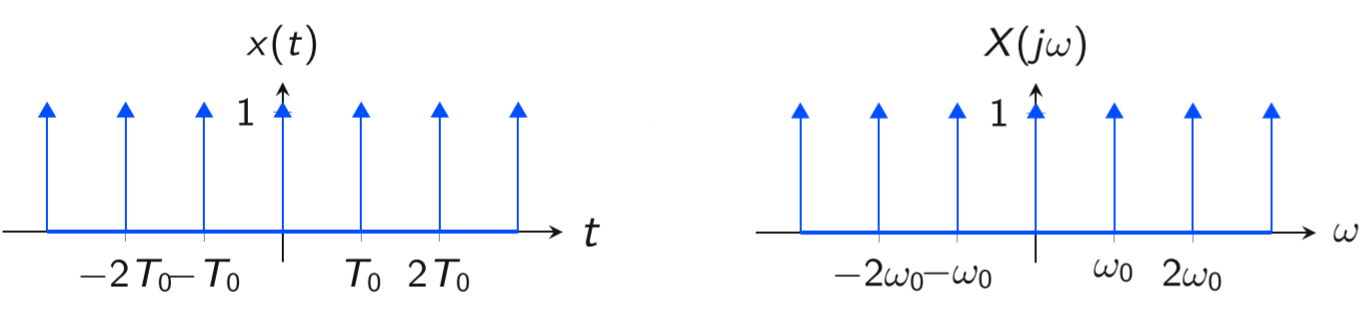
\includegraphics[width=7cm]{img/peigne.png}
\caption{peigne de Dirac (avec un petit spoil)}
\end{figure}
formellement un peigne de Dirac est:
\begin{equation}
x(t) = \sum_{k \in \mathbb{Z}} \delta(t-kT_0)
\end{equation}
et son $X(j\omega)$ est:
\begin{equation}
x(t) \longleftrightarrow X(j\omega) = \omega_0 x_{\omega_0} (\omega) \text{ avec } \omega_0 = \frac{2\pi}{T_0}
\end{equation}

\subsubsection{Preuve}
\begin{align*}
X(j\omega) &= \int_{-\infty}^{\infty} x(t) e^{-j \omega t} dt\\
&= \sum_{k = -\infty}^{\infty} \int_{-\infty}^{\infty} \delta(t- kT_0) e^{-j \omega t} dt\\
&= \sum_{k = -\infty}^{\infty} e^{-j \omega k T_0} \text{ car on a une énergie finie}\\
\mathcal{F}(\delta(t-kT_0)) &= e^{-j\omega k T_0}
\end{align*}
Ensuite, on va refaire une série de Fourier:
\begin{align*}
x(t) &= \sum_{l = -\infty}^{\infty} X_l e^{j\omega_0 t} & X_l &=  \frac{1}{T_0} \int_{-\frac{T_0}{2}}^{\frac{T_0}{2}} x(t) e^{-j \omega_0 lt} dt\\
&= \frac{1}{T_0} \sum_{l = -\infty}^{\infty} e^{j\omega_0 lt} & &= \frac{1}{T_0} \int \delta(t) e^{-j \omega_0 lt} dt= \frac{1}{T_0}
\end{align*} %pas sûr sûr pour cette démo je doisd recheck
Ensuite, on utilise la dualité:
\begin{align*}
x(t) &\longleftrightarrow X(j\omega)\\
X(jt) &\longleftrightarrow 2\pi x(-\omega)\\
\mathcal{F}(e^{j\omega_0 lt}) &= 2 \pi \delta(\omega - \omega_0 l)\\
x(t) = \frac{1}{T_0} \sum_{l = - \infty}^{\infty} 2 \pi \delta(\omega - l \omega_0) &= \omega_0 \sum (\delta(\omega -l \omega_0) = \omega_0 x(\omega)
\end{align*}

\subsection{Fonction échelon}
\begin{figure}[H]
\centering
\includegraphics[width=10cm]{img/echeF.png}
\caption{Transformé de la fonction échelon}
\end{figure}
Sa transformée de Fourier est:
\begin{equation}
x(t) = u(t) \longleftrightarrow X(j\omega) = \pi \delta(t) + \frac{1}{j \omega}
\end{equation}

\subsubsection{Preuve}
On utilise l'intégration car on sait que:
\begin{align*}
u(t) &=  \int_0^{\infty} \delta(t) dt\\
\mathcal{F}(\delta(t)) &= 1\\
u(j\omega) &= \frac{1}{j \omega} + \pi \delta(\omega)
\end{align*}

\subsection{Fonction fenêtre} \label{window}
Cette fonction, correspond à 2 impulsion. tel que:
\begin{equation}
\Pi = u(t+1) - u(t-1)
\end{equation}
Ces fonctions sont des filtres \textit{passes-bandes} et à pour transformé de Fourier:
\begin{align*}
x(t) = \Pi (t) \longleftrightarrow X(j\omega) = 2 sinc(t) = 2\frac{sin(\omega)}{\omega}
\end{align*}

\subsubsection{Preuve}
On utilise l'\textit{addition} de 2 échelons \textit{translatés}.
%Refaire toute la preuve

\subsection{Fonction signe}
La fonction signe est:
\begin{equation}
sign(t) = \begin{cases}
-1 \quad t < 0\\
0 \quad t = 0\\
1 \quad t > 0
\end{cases}
\end{equation}
et à pour transformée de Fourier:
\begin{align*}
x(t) = sign(t) = \longleftrightarrow X(j\omega) = \frac{2}{j\omega}
\end{align*}
Cela se prouve avec la dilatation et la translation de la fonction échelon.

\section{Tableau de Check}
\begin{center}
    \begin{tabular}{|m {5cm}| m {5cm}|}
    \hline
    \cellcolor[gray]{0.8} Domaine temporel &  \cellcolor[gray]{0.8} Domaine spectral \\ \hline
    $x(t) = u(t)$ & $X(j \omega) = \frac{1}{j\omega} + \pi \delta(\omega)$ \\\hline
    $x(t) = \delta(t)$ & $X(j \omega) = 1$ \\\hline
    $x(t) = 1$ & $X(j \omega) = 2\pi\delta(\omega)$ \\\hline
    $x(t) = \left\{\begin{aligned}
    1 \text{ si } |t| \leqslant T_0 \\
    0 \text{ sinon}
    \end{aligned}\right.
    $ & $X(j \omega) = \frac{2T_0\sin(\omega T_0)}{\omega T_0}$ \\\hline
    $x(t) = \frac{1}{t\pi}\sin(Wt)$ & $X(j \omega) = \left\{\begin{aligned}
    1 \text{ si } |\omega| \leqslant W \\
    0 \text{ sinon}
    \end{aligned}\right.$ \\ \hline
    $x(t) = e^{-at}u(t), \Re(a) > 0$ & $X(j\omega) = \frac{1}{a + j\omega}$\\\hline
    $x(t) = \sum_{n \in \mathbb{Z}} \delta(t-nT)$ & $X(j \omega) = \frac{2\pi}{T}\sum_{k\in\mathbb{Z}}\delta(\omega - k \frac{2\pi}{T})$ \\\hline
\end{tabular}
\end{center}
\subsubsection{Transformées de signaux discrets}
\begin{center}
    \begin{tabular}{|m {6cm}| m {6cm}|}
    \hline
    \cellcolor[gray]{0.8} Domaine temporel & \cellcolor[gray]{0.8} Domaine spectral \\  \hline
    $x[n] = u[n]$ & $X(e^{j\Omega}) = \frac{1}{1-e^{-j\Omega}} + \pi \sum_{p\in\mathbb{Z}} \delta(\Omega - 2\pi p)$ \\\hline
    $x[n] = \delta[n]$ & $X(e^{j\Omega}) = 1$ \\\hline
    $x[n] = \left\{\begin{aligned}
    1 \text{ si } |n| \leqslant M \\
    0 \text{ sinon}
    \end{aligned}\right.
    $ & $X(e^{j\Omega}) = \frac{\sin(\Omega(M + 1/2))}{\sin(\Omega/2)}$ \\\hline
    $x[n] = \frac{1}{n\pi}\sin(Wn), 0<W \leqslant \pi$ & $X(e^{j\Omega}) = \left\{\begin{aligned}
    1 \text{ si } |\Omega| \leqslant W \\
    0 \text{ sinon}
    \end{aligned}\right.$ \\ \hline
    $x[n] = \alpha^nu[n], |\alpha|<1$ & $X(e^{j\Omega}) = \frac{1}{1-\alpha e^{-j\Omega}}$\\ \hline
\end{tabular}
\end{center}

\chapter{L'échantillonnage}
L'échantillonnage est quelque chose qui est partout autour de nous. C'est le fait de transformer un signal continu (\textit{son, vidéo, ...}) en un signal discret. (afin de le stocker sur un pc, ...) C'est donc un processus vital à l'ère de l'informatique.
\section{Lien entre le continu et le discret}
Donc, pour sauvegarder un signal en discret, il faut \textit{ponctuellement} le sauvegarder. On appelle cela \textcolor{blue}{l'échantillonnage}

\subsection{L'échantillonnage}
\begin{wrapfigure}{r}{.5\textwidth}
\centering
\begin{align*}
\text{Pas d'échantillonnage: } &T_e\\
\text{Fréquence d'échantillonnage: }  f_e &= \frac{1}{T_e}\\
x[n] &= x(nT_e)\\
x_e(t)=x(t) \sum_{n \in \mathbb{Z}} \delta(t-nT_e)&= \sum_{n \in \mathbb{Z}} x(nT_e)\delta(t-nT_e)
\end{align*}
\end{wrapfigure}
On relève le signal discret toutes les $T_e$ secondes. Notre signal discret correspond à $x[n]$. Donc la transformation continu $\rightarrow$ est \textit{trivial}.\\
Une fois qu'on a notre signal \textit{discret}, on peu le retransformer en un signal discret ! En effet, on peut lier $x(t)$ à un peigne / train de Dirac.\\
On remarque que $x(nT_e) = x[n]$.

\subsubsection{Transformé de Fourier via continu}
Pour trouver la transformer de Fourier de notre $x_e(t)$ on réalise ceci:
\begin{align*}
x_e(t)&= x(t) \sum_{n \in \mathbb{Z}} \delta(t-nT_e)\\
X_e(j\omega) &= \frac{1}{2\pi} \Bigr[ X(j\omega) \ast \frac{2\pi}{T_e} \sum_{k \in \mathbb{Z}} \delta(\omega- \frac{2\pi}{T_e}k) \Big] \qquad  \frac{2\pi}{T_e} = \omega_e\\
&= \frac{1}{T_e} \Bigr[ X \ast \sum_{k \in \mathbb{Z}} \delta(-\omega_e) \Bigr](j\omega)\\
&= \frac{1}{T_e} \sum_{k \in \mathbb{Z}} X(j(\omega -k \omega_e))
\end{align*}
\newpage
\begin{wrapfigure}{r}{.5\textwidth}
\centering
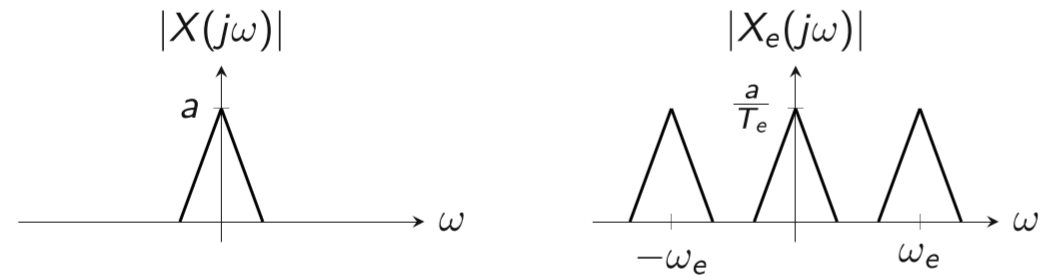
\includegraphics[width=7cm]{img/rep.png}
\end{wrapfigure}
Donc notre $\omega_e$ représente la période. On observe également une différence entre $|X(j\omega)|$ et $|X_e(j\omega)|$. En effet, on peut remarquer une répétition tous les $\omega_e = 2 \pi f_e$. Cette contrainte va être très importante pour le taux d'échantillonnage et pour le repli spectral (\ref{spec})

\subsubsection{Transformé de Fourier via discret}
\begin{align*}
x_e(t)&= \sum_{n \in \mathbb{Z}} x[n]\delta(t-nT_e)\\
X_e(j\omega) &= \sum_{n \in \mathbb{Z}} x[n] e^{-j \omega n T_e}\\
&= X(e^{j\Omega})\vert_{\Omega = \omega T_e}
\end{align*}
On retrouve également ce phénomène de \textit{répétition} pouvant mener à un enchevêtrement.

\begin{figure}[H]
\centering
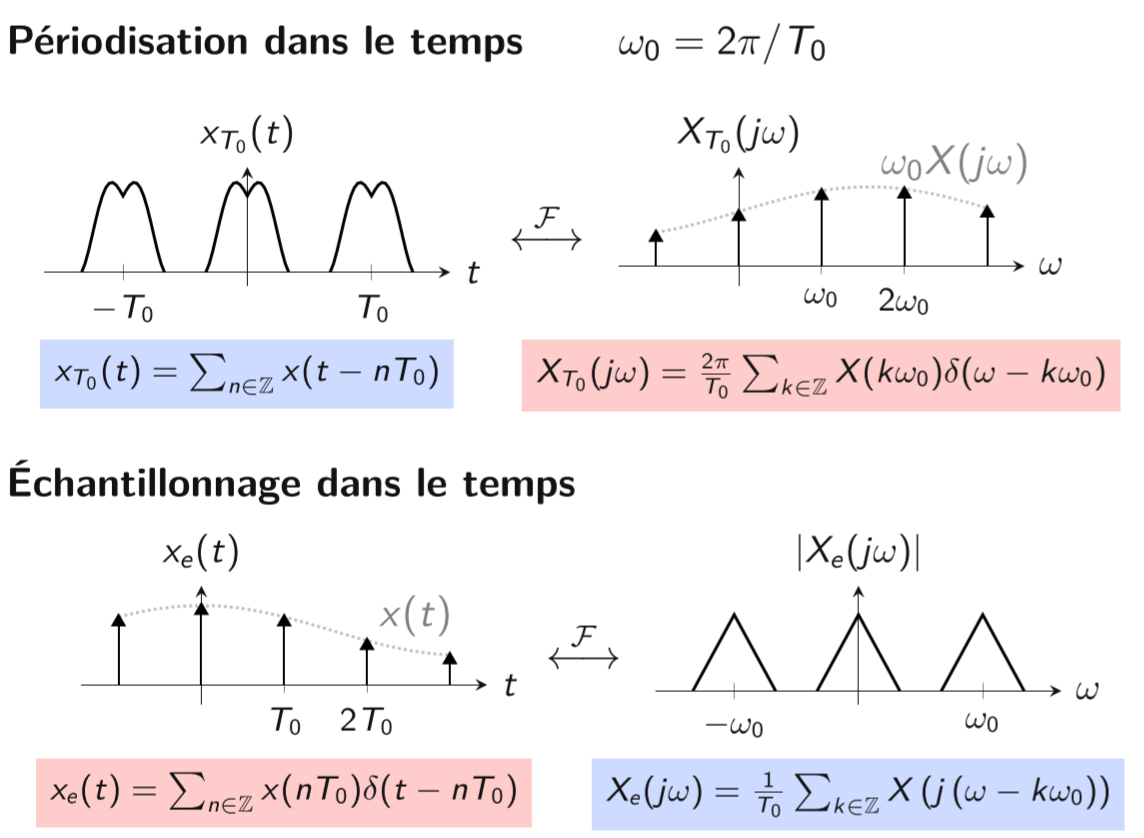
\includegraphics[width=10cm]{img/dua.png}
\caption{Dualité de Fourier}
\end{figure}

\section{Repli spectral} \label{spec}
Comme notre transformé de Fourier se répète tous les $\omega_e$, cela indique que le pas de temps \textit{d'échantillonnage} est primordial. Un pas trop \textit{petit} et les répétitions se \textcolor{red}{superposent}. On appelle cela le \textcolor{blue}{repli spectral} (\textit{aliasing}).\\
On peut penser aux roues d'un voiture, qui si le nombre de \textit{FPS} n'est pas assez élevé pour le nombre de rotation par seconde, nous donnera l'impression qu'elle tourne à l'envers.

\subsection{Bien échantillonner}
Avec l'idée de la \textit{voiture}, on peut déjà poser le fait qu'un bon échantillonnage est $2T_e \leq T$. Ainsi on verra la rotation.

\subsubsection{Théorème de Shannon} \label{Sha}
Une fonction (à bande limitée) qui ne contient pas de fréquences supérieures à $f_{max}$ est complètement déterminée par ses échantillons pour autant que:
\begin{align*}
f_e > 2 f_{max} \longleftrightarrow \omega_e > 2 \omega_{max}
\end{align*}	

\subsection{Reconstruire un signal}
Si le théorème de Shanon (\ref{Sha}) est bien respecté, on peut donc reconstituer un signal en \textit{continu} en filtrant son \textit{spectre discret}.

\begin{align*}
X(j\omega) = X_e(j\omega) T_e \sqcap \Bigr( \frac{\omega}{\omega_c} \Bigr) \qquad (\omega_{max} \leq \omega_c \leq \omega_e - \omega_{max})
\end{align*}

Il existe également une formule s'intitulant la \textcolor{blue}{formule de Shanon}. On rappelle que $x[n]$ correspond au signal échantillonné à un interval $T_e$:

\begin{align*}
\sum_{n \in \mathbb{Z}} x[n] sinc\Bigr( \frac{t-nT_e}{T_e} \Bigr)
\end{align*}
L'utilité du sinus \textcolor{blue}{cardinal} est qu'il interpole les points $(t, x(nT_e))$. Il existe d'autres fonctions d'interpolations qui donnent des résultats différents.
\begin{figure}[H]
\centering
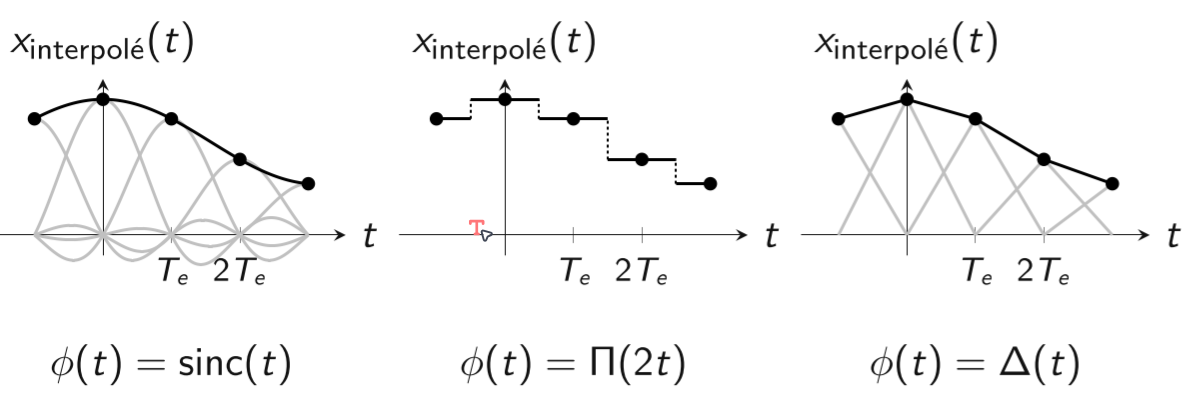
\includegraphics[width=10cm]{img/int.png}
\caption{Différentes interpolations}
\end{figure}

\subsection{Généralisation de Shanon}
Donc de manière plus général, on peut reconstruire tous signaux tant qu'il n'y a pas de recouvrement spectral. Par exemple des signaux plus complexes possédant \textbf{plusieurs} fréquences et qui sont de formes variées. On doit simplement respecter la formule de Shanon et bien lier la fréquence positive et sa fréquence négative. (\textit{dualité fréquentielle})

\section{Sur- et Sous-échantillonnage}
\begin{tabular}{| m{3cm} | m{5cm} | m{5cm} |}
\hline
\cellcolor[rgb]{0.8, 0.8, 0.8} & \cellcolor[rgb]{0.8, 0.8, 0.8} Variation du nombre d'échantillon sur une \textit{même} période & \cellcolor[rgb]{0.8, 0.8, 0.8} Variation de la durée de prise de donnée\\
\hline
\cellcolor[rgb]{0.8, 0.8, 0.8} Sous-échantillonnage & On a une même largeur de bande mais un rapprochement des spectres & On a une sorte de dilatation des spectres en phasorielles donc plus facile d'avoir de l'\textit{aliasing} même un même espacement entre les répétitions.\\ 
\hline
\cellcolor[rgb]{0.8, 0.8, 0.8} Sur-échantillonnage & Si on rajoute des données inutiles (ex: des 0) on a un rétrécissement des bandes mais un même espacement & On a une même bande des spectres et un rapprochement des spectres entre eux. \\
\hline
\end{tabular}

\chapter{Discrete Fourier Transform (DFT)} 
On est motivé à trouver la \textit{DFT} car sur les PC, on manipule que des signaux discrets. Donc on veut passer d'un signal continu à un signal discret, le manipuler et pouvoir le restituer en continu. De plus, un signal ne peut être infini.\\
Candidat:
\begin{enumerate}
\item Transformé de Fourier: signal x est \textcolor{blue}{continu} et sur un support \textcolor{blue}{infini}.
\item Série de Fourier: signal x est discrète et sur un support \textcolor{blue}{infini}.
\item Transformé de Fourier en temps discret: est \textcolor{blue}{continue}.
\item Série de Fourier discrète: on a besoin d'un signal discret \textcolor{blue}{périodique} et nous renvoie un signal \textcolor{blue}{périodique}
\end{enumerate}
Donc de ce qu'on a vu, rien ne fonctionne, on doit introduire une nouvelle \textit{transformée}, la \textbf{DFT} ou \textit{transformée de Fourier discrète}.

\section{Définition}
Depuis une suite \textit{M-périodique} $x[n]$ on construit une suite $X_{DFT}[k]$ qui est aussi \textit{M-périodique} et appelé la \textit{transformée de Fourier discrète} ou DFT de $x[n]$:
\begin{equation}
X_{DFT}[k] = \sum_{n=0}^{M-1}x[n]e^{-2\pi j k n /M}
\end{equation}
On peut aussi représenter cela via une matrice de Vandermonde:
\begin{equation}
\begin{bmatrix}
X_{DFT}[0]\\
X_{DFT}[1]\\
\vdots\\
X_{DFT}[M-1]
\end{bmatrix} =
\begin{bmatrix}
1 & 1 & \ldots & 1\\
1 & e^{-2\pi j \frac{1}{M}} & \ldots & e^{-2\pi j \frac{M-1}{M}}\\
\vdots & \vdots & \ddots & \vdots\\
1 & e^{-2\pi j \frac{M-1}{M}} & \ldots & e^{-2 \pi j \frac{(M-1)^2}{M}} 
\end{bmatrix}
\begin{bmatrix}
x[0]\\
x[1]\\
\vdots \\
x[M-1]
\end{bmatrix}
\end{equation}

Notre matrice de \textit{Vandermonde} est utilisée pour comparer les signaux. La \textbf{DFT} compare des signaux sous forme de vecteur entre eux\footnote{Bonne \href{https://youtu.be/yYEMxqreA10?t=1294}{vidéo} pour mieux comprendre cette idée}. Vandermonde possède toutes les fréquences possibles (définit par la M-périodicité) et compare avec notre signal de base. On aura une valeur \textbf{non-nulle} seulement pour des signaux qui sont en "\textbf{résonances}". 

\subsubsection{non-périodique}
Si $x[n]$ est \textbf{non-périodique} on va définir sa version périodisé.
\begin{align*}
x_M[n] &= \sum_{m \in \mathbb{Z}} x[n + mM]\\
X(e^{j\Omega_k}) &= \sum_{n\in \mathbb{Z}} x[n]e^{-2\pi j k n/M}\\
&= X_{M, DFT}[k]
\end{align*}
Et donc notre DTFT de $x[n]$ évaluée en $\Omega_k = 2\pi k / M$
\textcolor{red}{TODO démonstration}

\subsubsection{En pratique}
Ils existent 3 grandes familles de signaux qui nous intéressent pour la \textit{DFT}:
\begin{enumerate}
\item Signaux périodiques de période $M$
\item Signaux à support fini dans $\{0, ..., M-1\}$
\item Signaux à support infini.
\end{enumerate}
Donc pour le point 3, on doit \textit{tronquer} notre signal pour le périodiser.

\subsubsection{Zero padding}
C'est le principe du \textit{ré-échantillonnage} de la DTFT. On prend un signal x[n] qui a un support fini et non-périodique.\\
On va choisir une taille de périodisation $M'$ tel que $M'>M$ en rajoutant des zéros. On évalue donc la DTFT de $x[n]$ en d'autres fréquences.
\begin{figure}[H]
\centering
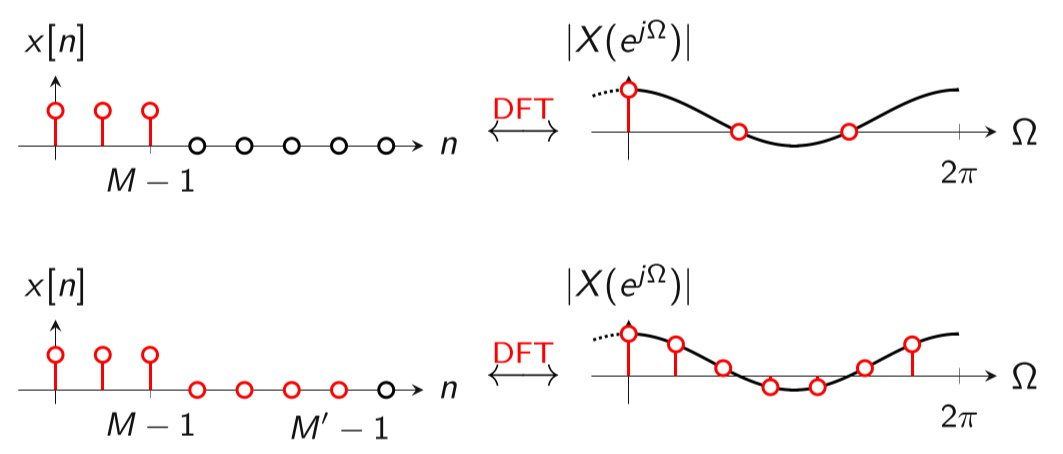
\includegraphics[width=8cm]{img/zero.png}
\end{figure}

\subsubsection{Propriétés de la DFT}

\begin{center}
\begin{tabular}{| m{2cm} | m{4cm} | m{4cm} |}
\hline
Opération &$x[n]$& $X_{DFT}[k]$\\
\hline
Combinaison linéaire & $\sum_i \alpha_i x_i[n]$ & $\sum_i \alpha_i X_{DFT,i} [k]; \alpha_i \in \mathbb{R}$ \\
\hline
Renversement & $x[-n]$ & $X_{DFT}[-k]$ \\
\hline
Complexe conjugué & $x[n]^{\ast}$ & $X_{DFT}[-k]^{\ast}$\\
\hline
Translation & $x[n-n_0]; n_0 \in \mathbb{Z}$ & $e^{-jk\frac{2\pi n_0}{M}}X_{DFT}[k]$ \\
\hline
Modulation & $e^{jk\frac{2\pi k_0}{M}}x[n]; k_0 \in \mathbb{Z}$ & $X_{DFT}[k-k_0]$ \\
\hline
Convolution cyclique & $\sum_{m=0}^{M-1}x_1[m]x_2[n-m]$ & $(X_{DFT,1}\cdot X_{DFT,2})[k]$ \\
\hline
Multiplication & $(x_1 \cdot x_2)[n]$ & $\frac{1}{M} \sum_{m=0}^{M-1} X_1[m]X_2[k-m]$ \\
\hline
Perseval & $\sum_{n=0}^{M-1} |x[n]|^2$ & $\frac{1}{M}\sum_{m=0}^{M-1}|X_{DFT}[k]|^2$ \\
\hline
\end{tabular}
\end{center}


\section{Transformée Rapide}
On doit en moyenne réaliser $8M^2$ opérations (avec $M$ la portée finie du signal)\\
En 1965, Cooley et Tukey ont proposé FFT ou \textit{Fast Fourier Transform} qui est basé sur la \textcolor{blue}{décimation temporelle}\\
Pour simplifier, on factorise $M$ et on divise la somme de la \textit{DFT} en sous-sommes qui correspondent à des DFT de plus petites tailles.


\chapter{Transformée de Laplace}
C'est une extension de la transformée de Fourier et permet de l'appliquer à plus de signaux (surtout des signaux courants dans le mone réel).

\subsection{Limitation}
On se souvient donc des transformées de Fourier (\ref{Fourier}). On peut ainsi réaliser des convolutions pour des systèmes via des multiplications en milieu fréquentiel. Cependant, on s'intéresse à des signaux ayant un début, un $0$
\subsubsection{Existence}
\begin{align*}
x(t) &= t 1(t)\\
\mathcal{F} (x) \longleftrightarrow \int_{-\infty}^{\infty} x(t) e^{-i \omega t} dt &= \int_0^{\infty} t e^{-i \omega t} dt = \left[ \frac{1 + i \omega t}{\omega^2} e^{-i \omega t} \right]_0^{\infty}
\end{align*}
On a un signal qui ne converge pas et oscille.

\subsection{Généralisation}
On peut utiliser un signal atténué ce qui permettrait de converger vers nul en l'infini et de même retrouver son résultat inverse:
\begin{align*}
x(t)e^{- \sigma t } &= t 1(t) e^{- \sigma t}\\
\mathcal{F} (x e^{- \sigma t}) \longleftrightarrow \int_{-\infty}^{\infty} x(t) e^{- \sigma t} e^{-i \omega t} dt &= \int_0^{\infty} t e^{-(\sigma + i \omega ) t} dt = \left[- \frac{1 + (\sigma + i \omega) t}{(\sigma + i \omega)^2} e^{-(\sigma + i \omega )t} \right]_0^{\infty}\\
X_{\sigma} (i \omega) &= \frac{1}{(\sigma + i \omega)^2}
\end{align*}
Pour retrouver le signal $x(t)$ sans la pré-multiplication, il faut réaliser cette opération
\begin{align*}
x(t) &= e^{\sigma t} \mathcal{F}-1 (X_{\sigma})\\
&= \frac{1}{2 \pi }\int_{-\infty}^{\infty} X_{\sigma} (i \omega) e^{\sigma t} e^{i \omega t} d\omega
\end{align*}
Ainsi, on peut s'assurer d'avoir une réponse pour nos systèmes. En effet, on va appliquer cette atténuation ainsi:
\begin{align*}
H\{e^{\sigma t} e^{i \omega t} \} &= h(t) \ast (e^{\sigma t} e^{i \omega t}) = H_{\sigma} (i \omega) e^{\sigma t} e^{i \omega t}
\end{align*}

\subsubsection{Simplification}
La notation courante de la \textit{transformée de Laplace} est $s = \sigma + i \omega$.
\begin{align*}
\int_{-\infty}^{\infty} x(t) e^{- \sigma t} e^{-i \omega t} dt = \int_{-\infty}^{\infty} x(t) e^{-( \sigma + i \omega) t} dt &= \int_{-\infty}^{\infty} x(t) e^{-( s) t} dt
\end{align*}

\section{Transformée}
La transformée de Laplace d'un signal $x$ est une généralisation de $s \in C$ de la transformée de \textit{Fourier}
\begin{align*}
X(s) = \mathcal{L}(x) := \int_{-\infty}^{\infty} x(t) e^{- s t} dt 
\end{align*}
$s$ est définie que sur la région où l'intégrale existe. On appelle cette région le \textbf{ROC} (\textit{Region of Convergence}).\\
La transformée inverse est définit ainsi:
\begin{align*}
x(t) = \mathcal{L}^{-1}(X) &:= \frac{1}{2 \pi} \int_{-\infty}^{\infty} X( \sigma + i \omega ) e^{(\sigma + i \omega)t } d \omega\\
&:= \frac{1}{2\pi} \int_{- \infty}^{\infty} X(s) e^{st} d\omega
\end{align*}
Et cela est valable pour tout $\sigma$ tel que $X$ est défini sur $\sigma + i \mathbb{R}$

\subsection{Région de Convergence et égalité}
Si $\mathcal{L}(x) = \mathcal{L}(y)$ sur $\sigma + i \mathbb{R}$ pour un $\sigma$ quelconque, alors $x=y$. Cependant, cela ne nous indique pas si $\mathcal{L}(x)$ et $\mathcal{L}(y)$ ont le même ROC.
\subsubsection{Exemple}
\begin{align*}
\mathcal{L}(1(t) e^t) &= \frac{1}{s-1} & \mathcal{L}(-1(-t) e^t) &= \frac{1}{s-1}\\
\mathfrak{R}(s) &> 1 & \mathfrak{R}(s) &< 1 
\end{align*}
Laplace est donc une fonction et un domaine de définition.

\subsubsection{Déterminer le ROC}
\begin{enumerate}
\item Si support fini $\rightarrow$ $ROC = \mathbb{C}$
\item Support fini à gauche et $|x(t)| < a e^{k_1 t}$ $\rightarrow$ $\mathfrak{R}(s) > k_1$
\item Support infini à droite, et $|x(t)| < a e^{k_2 t}$ $\rightarrow$ $\mathfrak{R}(s) < k_2$
\item support infini et borné à droite $|x(t)|< a e^{k_1 t}$ et à gauche $|x(t)| < a e^{k_2 t}$ $\rightarrow$ $k_1 < \mathfrak{R}(s) < k_2$
\end{enumerate}

\subsection{Propriétés}

\begin{center}
\begin{tabular}{|m{2.5cm}|m{7cm}|}
\hline
\textbf{Linéarité} & $\mathcal{L}(a_1 x_1 + a_2 x_2) = a_1 \mathcal{L}(x_1) + a_2 \mathcal{L}(x_2)$ \newline  ROC R: $R \supseteq R_1 \cap R_2$ \\
\hline
\textbf{Décalage temporel} & $\mathcal{L}(x(t-t_0)) = e^{-s t_0} \mathcal{L}(x(t))$ \newline même ROC\\
\hline
\textbf{Décalage fréquentiel} & $\mathcal{L}(e^{s_0 t}x(t)) = X(s-s_0)$ \newline ROC $= R + \mathfrak{R}(s_0)$\\
\hline
\textbf{Convolution} & $\mathcal{L}(x \ast y) = \mathcal{L}(x) \mathcal{L}(y) = XY$ \newline ROC $R$: $R \supseteq R_1 \cap R_2$\\
\hline
\textbf{Différentiation} & $\mathcal{L} \left( \frac{dx}{dt} \right) = s \mathcal{L}(x)$\\
\hline
\textbf{Intégration} & $\mathcal{L} \left( \int_{-\infty}^t x( \tau ) d \tau \right) = \frac{1}{s} \mathcal{L}(x)$\\
\hline
\textbf{Différentiation fréquentielle} & $\mathcal{L}(-tx(t)) = \frac{d}{ds} X(s)$\\
\hline
\end{tabular}
\end{center}
\subsection{En pratique}
Pour utiliser les transformées de Laplace, on utilise des logiciels, des tables ou les propriétés de linéarité.\\
On utilise à fond les décomposition en fraction simple et on utilise la linéarité sur des fonctions simplifier.

\section{Systèmes LTI: fonctions de transfert}
Si nous avons un système LTI $\mathcal{H}$ qui est entièrement caractérisé par une réponse impulsionnelle $h$. Sa réponse à une entrée $u$ est $y = h \ast u$. On réalise $Y(s) = \mathcal{L}(h \ast u) = H(s) U(s)$. La fonction de transfert est donc: \textbf{$H(s) = \mathcal{L}(h)$}. (cela est équivalent à la réponse impulsionnelle et caractérise entièrement le système)

\subsection{Passage à d'autres représentations}
\subsubsection{Équation différentielle}
\begin{align*}
\sum_{k=0}^N a_k \left( \frac{d^k}{dt} \right) y(t) &= \sum_{k=0}^M b_k \left( \frac{d^k}{dt} \right) u(t) & &\Leftrightarrow & \sum_{k=0}^N a_k s^k Y &= \sum_{k=0}^M b_k s^k U & &\Leftrightarrow & Y &= \frac{\sum_{k=0}^M b_k s^k}{\sum_{k=0}^N a_k s^k} U
\end{align*}
On voit que la partie à gauche de $U$ à la dernière équation équation correspond à $H$

\subsubsection{Représentation d'état}
\begin{align*}
\frac{d}{dt}x(t) &= A x(t) + B u(t) & sX &= AX + BU\\
y &= C x(t) + D u(t) & Y &= (C (sI - A)^{-1} B + D) U\\
\end{align*}
On a donc une fonction de transfert \textcolor{red}{unidimensionnel} si on a 1 entrée et 1 sortie. Le problème devient algébrique et peut être vu comme un problème statique / constant.\\
La réponse impulsionnelle est:
\begin{align*}
H(s) &= C(sI - A)^{-1} B + D\\
(sI - A) & \text{ Diagonale: } s - a_{ii} \text{ hors diagonale } - a_{ij}\\
(sI - A)^{-1} & \text{ Transposée des co-facteurs déterminants de matrice } (n-1) \times (n-1) \text{ pour polynômes } \leqslant n-1 \\
& \text{ou pour les polynômes d'ordre n } det(sI-A)\\
C(SI-A)^{-1} B + D & \text{ Fonction rationnelle plus un facteur } D
\end{align*}
Si un système admet une représentation d'état, alors $H(s)$ est rationnelle. Le dénominateur vaut $det(sI -A)$ d'ordre n et le numérateur est inférieur à $n$ si pas de $D$ sinon $n$.\par
Si le système est causal et $H$ est rationnel, on peut prouver que:
\begin{itemize}
\item L'ordre du dénominateur $\geqslant$ ordre numérateur
\item Égalité $\Leftrightarrow h(0) \neq 0$
\item Les zéros du dénominateur $det(sI - A) = $ valeurs propres de A.
\end{itemize} 

\subsubsection{Schéma bloc}
Ainsi, les blocs intégrateurs $\int$ devient simplement $\times \frac{1}{s}$. Les blocs différenciateurs $\frac{d}{dt}$ deviennent $\times s$

\section{Transformée de Laplace unilatérale}
Cela répond à 2 questions critiques:
\begin{enumerate}
\item Comment le signal doit-il être en $- \infty$ et sans condition initiale
\item Certaines fonctions n'ont pas de transformée de Laplace comme: $e^{at}$
\end{enumerate}
Le problème c'est $-\infty$, on va réaliser la transformée de \textcolor{blue}{Laplace unilatérale}:
\begin{equation}
X_+ (s) = \mathcal{L}_+ (x) := \mathcal{L}(1(t) x(t)) = \int_{0^-}^{\infty} x(t) e^{st} dt
\end{equation}
Donc bien depuis $0^-$ (surtout quand on a $\delta (t)$). On a beaucoup de propriétés héritées de $\mathcal{L}$.\\
Faire son inverse permet de \textit{seulement} retrouver \textbf{$1(t) x(t)$} (on perd de l'information).

\subsection{propriétés}
\subsubsection{Convolution} 
\begin{equation}
\mathcal{L}_+ (x \ast y) \neq \mathcal{L}_+ (x) \mathcal{L}_+ (y)
\end{equation} 
Dans \textit{la plupart du temps}, mais on peut simplifier en \textbf{système causal} ($h(t) = 0 $ pour $t < 0$ ou bien le système est au repos)
\begin{equation}
\mathcal{L}_+ (y) = \mathcal{L}_+ (h) \mathcal{L}_+ (u) = H_+ \mathcal{L}_+ (u)
\end{equation}
Donc on va assumer, en \textcolor{red}{causal}, $H = H_+$

\subsubsection{Dérivation} \label{Dérivation}
\begin{equation}
\mathcal{L}_+ (x'(t)) = \int_0^{\infty} x'(t) e^{-st}dt = -x(0) + s X_+ (s)
\end{equation}
On remarque qu'on inclut bien les \textbf{conditions initiales} du système.

\subsubsection{Intégration}
\begin{equation}
\mathcal{L}_+ \left( \int_0^t x(\tau ) d \tau \right) = \frac{1}{s} \mathcal{L}_+ (x)
\end{equation}
Pour le prouver, on utilise le résultat de la dérivation vu en \ref{Dérivation}. De plus, $\int_0^0 x(\tau ) d \tau = 0$

\subsubsection{Limite de $X_+(s)$}
\begin{align}
\lim_{s \rightarrow 0} s X_+ (s) &= x(\infty) & \lim_{s \rightarrow + \infty} s X_+ (s) &= x(0^+)
\end{align}
Preuve \textit{informelle}:
\begin{align*}
\mathcal{L}_+ (x') &= s \mathcal{L}_+ (x) - x(0)\\
\lim_{s \rightarrow 0} sX_+ (s) &= x(0) + \lim_{s \rightarrow 0} \mathcal{L}_+ (x')(s)
& \approx x(0) + \int_0^{\infty} x'(t) e^{0.t} dt = x(\infty)
\end{align*}
Donc dans un système \textbf{stable} et \textbf{causal}, $H(0)$ représente le rapport entre la sortie et l'entrée à l'\textit{infini} ou après stabilisation.\\
On parle de gain à fréquence nulle ou \textit{steady-state}


\subsection{Résolution d'EDO}
\subsubsection{Exemple}
\begin{align*}
y'' + 3y' + 2y &= a1(t) & (s^2 + 3 s + 2)Y &= \frac{a}{s}
\end{align*}
La partie à droite correspond à l'EDO dans le domaine de Laplace. Nos conditions initiales sont: $y(0) = 0$ et $y'(0) = 0$
\begin{align*}
Y = \frac{a}{s(s^2 + 3s +2)} &= \frac{a}{2s} - \frac{a}{s+1} + \frac{a}{2(s+2)}\\
y(t) &= 1(t) a \left(\frac{1}{2} - e^{-t} + \frac{1}{2} e^{-2t} \right)
\end{align*}
On remarque que:
\begin{enumerate}
\item Les exposants des exponentielles correspondent aux racines du polynômes au dénominateur
\item Nous avons un "\textit{taux}" 0 de u
\item Ce sont les racines du polynômes caractéristiques
\end{enumerate}
\underline{Via Laplace unilatérale :}
\begin{align*}
(s^2 Y - sy_0 -y_0') + (3 sY -3 y_0) + (2Y) &= \frac{a}{s} & (s^2 + 3s + 2)Y &= \frac{a}{s} + (3-s) y_0 + y_0'\\
\end{align*}
\begin{equation}
Y = \textcolor{blue}{\frac{a}{s(s^2 + 3s + 2)}} + \frac{y_0 (3-s)}{s(s^2 + 3s + 2)} + \frac{y_0'}{s(s^2 + 3s +2)}
\end{equation}
En bleu, on a la réponse \textbf{forcée} (comme si on imposait que $y_0 = y_0' = 0$). Le reste de l'équation correspond à la réponse \textbf{libre} qui dépend des racines du polynômes caractéristiques et est linéaire en $y_0$ et $y_0'$.\par
On finit par réaliser la transformée inverse:
\begin{equation}
y(t) = 1(t) (\frac{a}{2} + (2 y_0 + y_0' -a ) e^{-t} + (\frac{a}{2} -y_0 -y_0') e^{-2t})
\end{equation}
Long mais programmable en calculant les racines du polynôme et en réduisant en fractions simples.


\chapter{Transformée en Z}
C'est l'équivalent en \textit{temps discret} de la \textit{transformée de Laplace}.
\section{Transformée en Z}
On fait face aux mêmes problèmes qu'avant mais ici pour la DTFT. On va donc partir de celle-ci et l'\textit{atténuer}. On ne fait plus la DTFT pour $x[n]$ mais pour $x[n]r^{-n}$
\begin{align*}
X_r(e^{i \omega}) &= \sum_{k = - \infty}^{\infty} x[k] r^{-k} e^{-i \omega k}\\
& = \sum_{k = - \infty}^{\infty} x[k] z^{-k}\\
DTFT^{-1} & \rightarrow x[n] r^{-n}
\end{align*}

\subsection{Convergence}
\begin{wrapfigure}{r}{.5\textwidth}
\centering
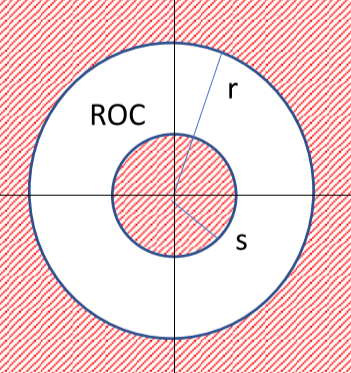
\includegraphics[width=6cm]{img/ROCLaurent.png}
\end{wrapfigure}
En simplifiant $z = r e^{i \omega}$ on peut réaliser ceci:
\begin{align*}
\mathcal{Z}\{x\} := X(z) &= \sum_{k = - \infty}^{\infty} x[k] z^{-k} \\
& = \sum_{k' = - \infty}^{\infty} x[-k'] z^{k'}
\end{align*}
Donc on transforme la transformé en Z en une \textbf{série de Laurent} avec $a_k = x[-k]$. On va séparer le tout en un anneau avec une partie intérieure et extérieure.
\begin{equation}
f(z) = \sum_{k \geqslant 0} a_k z^k + \sum_{k \leqslant -1} a_k z^k
\end{equation}
Il existe donc une convergence sur $A(0,r,s)$ comme ci-contre. $r$ est le rayon de convergence des $a_k$ tel que $r = sup\{\rho : \exists M: a_k \rho^k < M, \forall k > 0 \}$. On a également $1/s$ qui est le rayon de convergence de $a_{-k}$ comme $\frac{1}{s} = sup\{\rho : \exists M : a_{-k} \rho^k < M, \forall k > 0 \}$.\par
En particulier si $|a_k| < A \rho^{-k}$ et $|a_{-k}| < A' \sigma^{-k}$ pour $k > 0$ assez grand. On a donc une convergence pour tout $z \in A \left( 0, \rho, \frac{1}{\sigma} \right)$. Il existe donc un nombre \textit{fini} de $a_{-k} : \sigma = \infty$ et $A(0, \rho, 0)$. On a un nombre fini de $a_k : \rho = \infty$ et $A\left( 0, \infty , \frac{1}{\sigma} \right)$\\

Pour obtenir une sorte de série de Laurent, on doit réaliser cela:
\begin{equation}
X(z) = \sum_{k \geqslant 0} x[-k]z^k + \sum_{k \leqslant -1} x[-k] z^k
\end{equation}
Cela converge sur un anneau $A(0, r, s)$. $a_k$ devient $x[-k]$ et $a_{-k}$ devient $x[k]$. Le $\sigma$ indique un \textit{support fini dans le \textbf{futur}} et le $\rho$ est un \textit{support fini dans le \textbf{passé}}.

\subsubsection{Coefficient de la série}
Dans une série de Laurent et en transformée inverse:
\begin{align*}
a_k &= \frac{1}{2 \pi i} \int_{\partial B(0, \rho)} \frac{f(z)}{z^{k+1}} dz & x[-k] &= \frac{1}{2 \pi i} \int_{\partial B(0, \rho)} \frac{X(z)}{z^{k+1}} dz
\end{align*}
On a que pour n'importe quel $\rho \in (r,s)$
\begin{equation}
x[k] = \frac{1}{2 \pi i} \int_{\partial B(0, \rho)}X(z)z^{k-1} dz 
\end{equation}
On développe le tout:
\begin{align*}
& = \frac{1}{2 \pi i} \int_{- \pi}^{\pi} X(\rho e^{i \omega})(\rho e^{i \omega})^{k-1} i \rho e^{i \omega} d\omega\\
x[k] &= \frac{1}{2 \pi} \int_{- \pi}^{\pi} X(\rho e^{i \omega})\rho^k e^{i \omega k} d\omega
\end{align*}
On se rend compte que le signal $x[k]$ est un combinaison linéaire de $z^k = \rho^k e^{i \omega k} : \rho$ fixe et $\omega \in [-\pi, pi]$. \par
$X(z)$ est le coefficient de développement en signaux $z^k$ pour un $|z| = \rho$ fixé.

\subsubsection{Série de Laurent inverse} 
Si on a une fonction \textit{analytique} sur $\mathbb{C}$ sauf pour quelques points $c_1, c_2, ...$ Alors, il faut prendre l'anneau le plus grand.
\textcolor{red}{Rajouter plus de précisions}

\subsection{Propriétés}
\subsubsection{Linéarité}
\begin{align*}
\mathcal{Z}\{\alpha x + \beta y \} &= \alpha \mathcal{Z}\{x\} + \beta \mathcal{Z}\{y\} & ROC R: R \supseteq R_x &\cap R_y
\end{align*}

\subsubsection{Décalage temporel} \label{Ztemp}
\begin{align*}
\mathcal{Z}\{x[n -n_0]\} &= \sum_n x[n-n_0]z^{-n} \text{ changement de variable: } l = n - n_0\\
&= \sum_l x[l]z^{-(l+n_0)}\\
&= z^{-n_0} \sum_l x[l]z^{-l}\\
&= z^{-n_0} \mathcal{Z}\{x[n]\} \text{ même ROC}
\end{align*}

\subsubsection{Mises à l'échelle \textit{fréquentielle}}
\begin{align*}
X(az) &= \sum_n x[n](az)^{-n} \text{  ROC: scaling par } \frac{1}{|a|}\\
&= \sum_n (x[n] a^{-n}) z^{-n} = \mathcal{Z}\{a{^-n}x\}
\end{align*}

\subsubsection{Convolution}
\begin{align*}
\mathcal{Z}\{x \ast y \} &= \sum_k ( x \ast y)[k] z^{-k} = \sum_k \sum_l x[l] y[k-l]z^{-k}\\
&= \sum_k \sum_l x[l]z^{-l} y[k-l]z^{-k-l} \text{ Changement de variable: } k' = k-l\\
&= \sum_k \sum_l x[l]z^{-l} \sum_{k'} y[k']z^{-k'} = \mathcal{Z}\{x\} \mathcal{Z}\{y\}
\end{align*}

\subsubsection{"dérivée"}
Pas trop de sens, mais on réalise l'opération $\mathcal{Z}\{x[n+1]\}$ pour faire la "\textit{dérivé}". (\ref{Ztemp})

\subsubsection{Intégrale}
On réalise une sorte d'accumulation $y[n] = \sum_{k=-\infty}^n x[k]$, cela donne:
\begin{align*}
x[n] &= y[n] - y[n-1] & X &= (1- z^{-1})Y & Y &= \frac{1}{1 -z^{-1}} X 
\end{align*}

\subsubsection{Dérivée "fréquentielle"}
\begin{align*}
X'(z) &= - \mathcal{Z}\{x[n-1](n-1\} & \mathcal{Z}(nx[n]) &= -z X'(z)
\end{align*}

\subsection{Calcul pratique}
On utilise des logiciels, tables de transformés et on exploite la \textit{linéarité}. Ne pas oublier de décomposer en \textit{fraction simple}.


\section{Transformée en Z unilatérale}
\subsection{Motivation et Définition}
\begin{equation}
X_+ (z) = \mathcal{Z}_+ \{x\} := \mathcal{Z}_+ \{1x\} = \sum_{n=0}^{\infty} x[n] z^{-n}
\end{equation}
On réalise cela car pour des signaux de type $a^n$, on n'a généralement pas de convergence. (pour se convaincre on peut réaliser la transformée en Z)

\subsection{Propriétés}
\subsubsection{Convolution}
\begin{equation}
\mathcal{Z}_+ \{x \ast y\} \neq \mathcal{Z}_+ \{x\} \mathcal{Z}_+ \{y\}
\end{equation}
Si notre système est causal: $h[k] = 0$ pour $k < 0 \rightarrow \mathcal{Z}_+ (h) = \mathcal{Z}(h) = H$.\par
Si notre système est au repos en $k=0$ et l'entrée est nulle pour $k<0$ alors:
\begin{align*}
u[k] &= 1[k] u[k] & y[k] &= 1[k]y[k] & \mathcal{Z}_+ (y) &= \mathcal{Z}(y) & \mathcal{Z}_+ (u) &= \mathcal{Z}(u)
\end{align*}
Ce qui nous donne:
\begin{equation}
\mathcal{Z}_+ (y) = \mathcal{Z}_+ (h) \mathcal{Z}_+ (u) = H_+ U_+
\end{equation}
Si un système est supposé causal, $H = H_+$

\subsubsection{Décalage arrière}
\begin{equation}
\mathcal{Z}_+ \{x[n-1]\} = z^{-1} \mathcal{Z}_+ \{x[n]\} + x[-1]
\end{equation}

\subsubsection{Décalage avant}
\begin{equation}
\mathcal{Z}_+ \{x[n+1]\} = z \mathcal{Z}_+ \{x[n]\} - zx[0]
\end{equation}

\subsubsection{Limites}
\begin{align*}
\lim_{|z| \rightarrow \infty} X_+(z) &= x[0] & \lim_{z\rightarrow 1}(z-1) X_+(z) &= \lim_{n \rightarrow \infty} x[n]
\end{align*}

\subsubsection{Gain DC et steady-state}
Comme $Y_+ = HU_+$
\begin{equation}
\frac{y[\infty]}{u[\infty]} = \frac{\lim_{z\rightarrow 1}(z-1) Y_+(z)}{\lim_{z\rightarrow 1}(z-1) U_+(z)} = \lim_{z \rightarrow 1} \frac{(z-1) Y_+(z)}{(z-1) U_+(z)} = H(1)
\end{equation}
On réalise un décomposition du signal:
\begin{equation}
x[k] = \frac{1}{2 \pi i} \int_{\partial B(0, \rho)} X(z) z^{k-1} dz
\end{equation}
Si $\rho = 1$ donne une partie constante du signal. Donc $H(1)$ à un effet sur la partie constante du signal.
\par En temps continu:
\begin{equation}
x(t) = \frac{1}{2 \pi} \int_{\infty}^{\infty} X( \sigma + i \omega) e^{(\sigma + i \omega) t} d \omega
\end{equation}
Même conclusion qu'en discret.



\part{Systèmes}

\chapter{Système LIT}
Un système est une entité qui prend \textit{un ou plusieurs signaux} en entrée et produit \textit{de nouveaux signaux} en sortie.\\
Exemple: $H\{x[n]\} = x[n] + x[n-1]$. Un système est par exemple: \textit{une radio, une caméra, une voiture, ...}

\section{LIT}
Un système \textit{Linéaire et Indépendant du Temps} ou \textbf{LIT} est, comme son nom l'indique, linéaire donc:
\begin{equation}
\mathcal{H}\{a_1x_1 + ... + a_Nx_N\} = a_1\mathcal{H}\{x_1\} + ... + a_N\mathcal{H}\{x_N\} 
\end{equation}
Et un système est \textit{invariant temporelle} donc:
\begin{equation}
\begin{cases}
\mathcal{H} \text{ est invariant si } \forall t_0 \in \mathbb{N}\\
\mathcal{H}\{x\}[n] = y[n] \Rightarrow \mathcal{H}\{x[n-n_0]\} = y[n-n_0]
\end{cases}
\end{equation}
On remarque qu'on peut ré-écrire tous signaux via une somme d'impulsions. De plus, si $\mathcal{H}$ est linéaire alors:
\begin{equation}
\mathcal{H}\{x\} = \mathcal{H}\biggl\{\sum_{k= -\infty}^{\infty} x[k]\delta[n-k] \biggl\} = \sum_{k=-\infty}^{\infty} x[k]\mathcal{H}\{\delta[n-k]\}
\end{equation}
Si $\mathcal{H}$ est \textit{invariant} au temps et qu'on pose $h := \mathcal{H}\{\delta\}$
\begin{align*}
\mathcal{H}\{\delta[n-k]\} = \mathcal{H}\{\delta\}[n-k] &= h[n-k]\\
\mathcal{H}\{x\} = \sum_{k=-\infty}^{\infty} x[k]h[n-k] &=: x \ast h
\end{align*}
A noter que "$\ast$" fais référence à la convolution, sujet abordé à la section \ref{convo}.\\

Il est important de noter que toutes ces propriétés et caractéristiques des systèmes \textit{LIT} en \textbf{temps discret} sont également valables et ont un équivalent en \textbf{temps continu}.


\section{Réponse impulsionnelle}
La réponse impulsionnelle d'un système \textit{LIT} $\mathcal{H}$ est la réaction du système à une \textit{impulsion d'entrée} ($\delta[0]$) on le note $h$.\\

Pour \textbf{tout} système \textit{LIT}, le signal de sortie est le résultat de la convolution entre \textit{le signal d'entrée} et \textit{la réponse impulsionnelle}. Cela est d'autant plus utile grâce au propriété d'un tel système et sa linéarité.
\begin{align}
y[n] &= x[n] \ast h[n]\\
y(t) &= y(t) \ast h(t)
\end{align}

\subsubsection{Réponse indicielle}
C'est comme la \textit{réponse impulsionnelle} mais quand on fait passer un \textbf{échelon} dans notre système.

\subsubsection{Réponse fréquentielle}
Pour établir cette réponse, on applique un transformée de Fourier à la réponse impulsionnelle \textbf{OU} on utilise la propriété de convolution et multiplication:
\begin{align*}
H(j \omega) &= \mathcal{F}(h(t))\\
H(j \omega) &= \frac{Y(j \omega)}{X(j \omega)}
\end{align*}
Pour plus d'informations sur les réponse fréquentielles, il faut aller voir \ref{Bode}.

\section{Type de système}
\begin{center}
\begin{tabular}{|m{4cm}|m{10cm}|}
	\hline
	Système sans mémoire & Si la sortie du système \textit{à un temps donné} ne dépend que de l'entrée à \textbf{cet instant}.\\
	\hline
	Système causal & Le système \textbf{ne dépend pas} de ce qui se passe dans le \textit{futur}\\
	\hline
	Système stable ou (\textit{BIBO}) & Entrée \textit{bornée} donne une sortie \textit{bornée}\\
	\hline
	Système inversible & On sait \textit{retrouver} l'entrée en ayant la \textit{sortie}.\\
	\hline

\end{tabular}
\end{center}

\section{Modélisation et représentation des systèmes}
Comme vu précédemment, la réponse impulsionnelle est le résultat du système étant perturbé par une impulsion. 
\subsection{Inconvénient}
\begin{enumerate}
\item Fonction de taille \textit{infinie} et représentation donc \textit{peu simple}.
\item La modélisation d'un système ne mène généralement pas à une réponse impulsionnelle.
\item On doit connaitre l'entrée depuis $-\infty$.
\end{enumerate}


\subsection{Représentation}
\begin{wrapfigure}{r}{.3\textwidth}
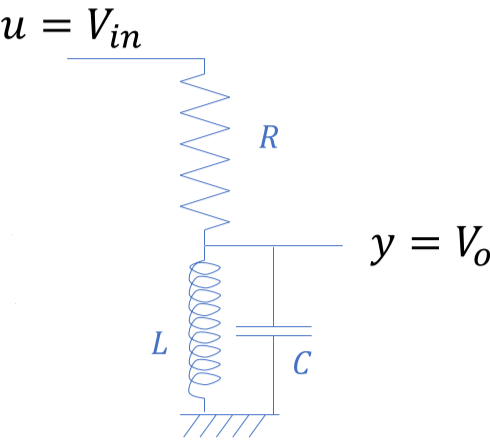
\includegraphics[width=5cm]{img/RLC.png}
\caption{Circuit RLC}
\label{fig:RLC}
\end{wrapfigure}
Il existe 3 grandes façons de représenter un système. Tout d'abord la méthode \textit{équation différentielle d'entrée-sortie}. Pour la suite des exemples, j'utiliserai un circuit \textit{RLC} comme montré ci-contre.\\

\textit{équation différentielle d'entrée-sortie} est une somme des dérivées comme montré dans l'équation \ref{eqn:es}. C'est plutôt facile de trouver les équations mais on fait face à un problème, l'opération \textit{dérivée} n'existe pas dans le monde réelle, il faut un opérateur intégrateur.\\

Ensuite, nous avons la \textit{représentation d'état} qui utilise des matrices pour former les équations différentielles comme nous voyons à l'équation \ref{eqn:mat}\\

La dernière représentation type est le \textit{schéma bloc} qui est visuel et qui utilise lui des blocs intégrateurs au lieu de dérivé comme montré à la figure \ref{fig:bloc}.

\begin{equation} \label{eqn:es}
\ddot{y} + \frac{1}{CR}\dot{y} + \frac{1}{LC}y = \frac{1}{CR}\dot{u}
\end{equation}

\begin{equation} \label{eqn:mat}
\frac{d}{dt}\begin{pmatrix}
V_0\\
I_L
\end{pmatrix} = \begin{pmatrix}
-1/RC & -1/C\\
1/L & 0
\end{pmatrix} \begin{pmatrix}
V_0\\
I_L
\end{pmatrix} + \begin{pmatrix}
1/RC\\
0
\end{pmatrix} u
\end{equation}

\begin{figure}[H] 
\centering
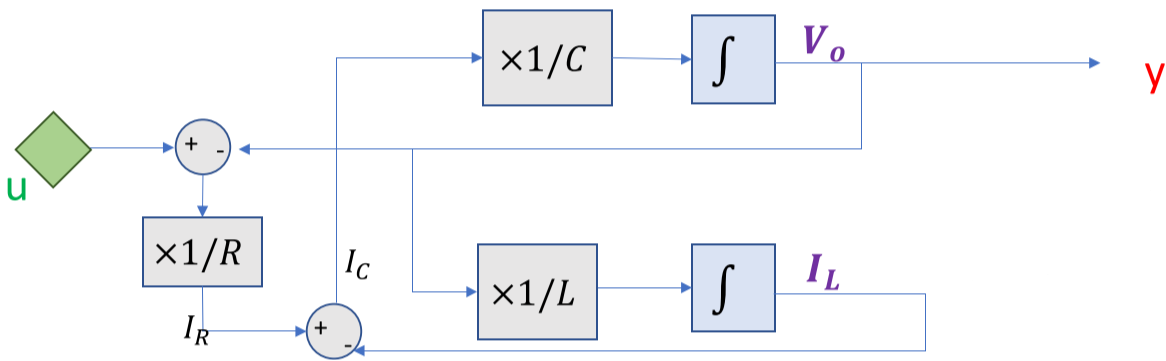
\includegraphics[width=7cm]{img/bloc.png}
\caption{Repésentation \textit{bloc} du système à la figure \ref{fig:RLC}}
\label{fig:bloc}
\end{figure}

\subsection{Équation différentielle entrée-sortie}
La forme générale de ces équations est de ce type:
\begin{equation}\label{eqn:difes}
\sum_{k = 0}^{N} a_k (\frac{d^k}{dt^k}) y(t) = \sum_{k = 0}^M b_k (\frac{d^k}{dt^k}) u(t)
\end{equation}
Quelque chose à bien remarquer est que ces équations ne modélisent \textit{qu'une partie} d'un système \textit{LIT}. Par exemple, on ne peut pas représenter un \textit{délai} ce qui est également rare dans la réalité.\\

Une chose à remarquer est que l'opérateur \textit{dérivé} peut se "\textit{démultiplier}" et possède une \textit{associativité} et \textit{commutativité}. Ainsi, on peut avoir une représentation dite "\textit{polynomiale}" comme ci-dessus qui est une autre écriture de l'équation \ref{eqn:difes}.
\begin{equation}\label{eqn:poly}
p(\frac{d}{dt})y(t) = q (\frac{d}{dt})u(t)
\end{equation}
Puis après, pour résoudre ce genre d'équation, on utilise des méthodes classiques vu au cours d'Analyse donc, solution homogène et particulière ...

\subsubsection{Réponse libre et forcée}
Une réponse \textit{libre} est la solution de l'équation homogène, donc quand $u(t) = 0$ à l'équation \ref{eqn:poly} et on garde les \textbf{mêmes conditions initiales}. En somme c'est la représentation de l'impact des \textit{CI}.\\

Une réponse \textit{forcée} est l'équation \ref{eqn:poly} mais avec les \textit{conditions initiales} nulles. Donc on s'intéresse à l'impact de l'entrée sans les conditions initiales. La somme de la réponse \textit{libre} et \textit{forcée} nous donne la réponse générale.

\subsubsection{Stabilité}
On peut avoir une intuition sur la stabilité de notre système en posant $y_H(t)$ qui équivaut à:
\begin{equation}
y_H(t) = \sum_i \alpha_ie^{r_it} \rightarrow \quad r_i \text{ correspond aux racines de p(z) de \ref{eqn:poly}}
\end{equation}
Si la partie réelle de $r_i < 0 \forall i$ alors on a une exponentielle décroissante donc \textbf{stable}. On appelle ce genre de système \textit{BIBO} stable ou \textit{Bounded Input Bounded Output}.\\

En revanche, si $r_i > 0 \exists i$ donc on a au moins une exponentielle croissante créant une \textit{instabilité}.\\

Si $r_i = 0 \exists i$ on dit qu'on a une \textit{stabilité marginale} ou \textit{instabilité}. Cela dépendera de la \textbf{multiplicité} et de \textbf{$te^{r_it}$}.

\subsubsection{Linéarité de l'entrée}
Avec cette représentation polynomiale, on peut facilement voir qu'on a une linéarité de l'entrée nous permettant de simplifier différent calcul. %rajouter la formule etc

\subsubsection{Avantages et Inconvénients}
2 représentations qui sont \ref{eqn:difes} et \ref{eqn:poly}. Les avantages:
\begin{itemize}
\item Représentation compacte.
\item Conditions initiales claires.
\item Facile de la transformer dans d'autres représentations.
\end{itemize}
Les désavantages:
\begin{itemize}
\item On peut perdre la représentation physique.
\end{itemize}

\subsection{Schéma Bloc}
Comme son nom l'indique, le schéma bloc utilise des "\textit{blocs}" pour représenter notre système. Ci-dessus on peut voir les composants de base composant ce type de schéma
\begin{figure}[H]
\centering
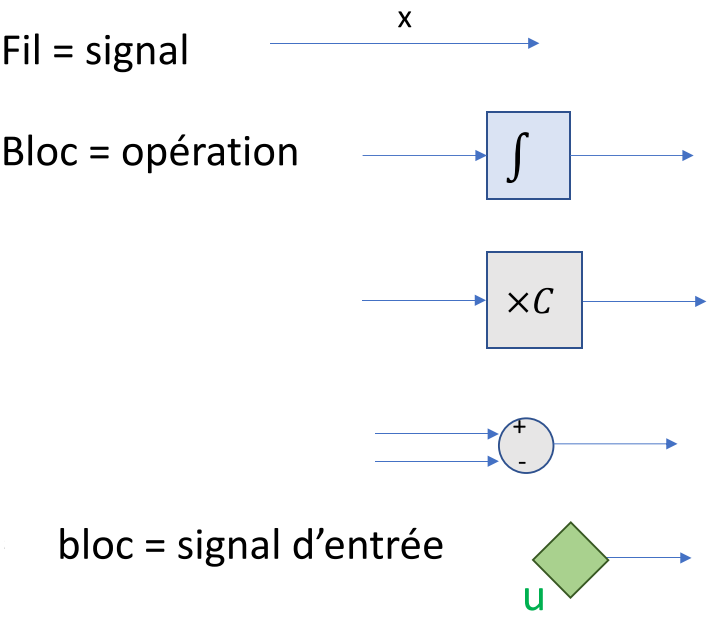
\includegraphics[width=5cm]{img/blocExemple.png}
\caption{Liste reprenant les blocs de base}
\end{figure}
Dans le cadre des systèmes \textit{LIT}, on se restreint souvent à l'addition, multiplication et intégration. On ne réalise que des opérations \textit{linéaires}.

\subsubsection{Avantages et Inconvénients}
Les avantages:
\begin{itemize}
	\item Représentation très intuitive.
	\item Proche de l'implémentation réelle du système.
	\item On peut plus facilement réfléchir sur le \textit{design} de notre système.
	\item Très modulaire.
\end{itemize}
Les désavantages:
\begin{itemize}
	\item Lien moins clair avec la solution.
\end{itemize}
De plus, on peut voir comme un \textit{avantage} ou \textit{inconvénient} le fait de pouvoir voir l'évolution des signaux entre chaque bloc plutôt qu'une sorte de boite noire "\textit{entrée-sortie}". On peut également réaliser de bien des manières des circuits.

\subsection{Représentation d'état}
Dans ce type de représentation, on a un \textcolor{red}{état $x$} qui est un \textit{vecteur} comportant toutes les infos internes de notre système. On a une  \textcolor{red}{entrée $u$} qui est un \textit{signal} extérieur affectant le système. Finalement on a une \textcolor{red}{sortie $y$} qui est un signal qu'on peut accéder depuis l'extérieur.\\
\begin{equation}
\begin{cases}
\text{évolution: }\frac{d}{dt}x(t) =  Ax(t) + Bu(t)\\
\text{sortie: } C x(t) + D u(t)
\end{cases}
\end{equation}

\subsubsection{Solution}
La solution \textit{homogène} de $e^{\lambda_it}$ avec $\lambda_i$ étant les valeurs propres de l'équation. Si la partie réelle des racines est négative pour tout $\lambda_i$.

\subsubsection{État non-unique}
Avec cette représentation, on peut facilement modifier les vecteurs et signaux pour rendre les équations plus simples. Cela n'a aucun impacte et rend les équations plus logiques pour un certain sens "\textit{réel}".
\begin{equation} \label{eqn:nonunique}
\begin{cases}
z = Tx \Rightarrow \frac{d}{dt}z = T\frac{d}{dt}x = TAT^{-1}z(t) + TBu(t)\\
y = Cx(t) + Bu(t) = CT^{-1}z(t) + Du(t) 
\end{cases}
\end{equation}

Si la matrice $A$ est diagonalisable, on peut réaliser un \textbf{découplage} et obtenir ainsi un mode dit \textit{découplé}. On peut également faire des \textit{blocs de Jordan} pour diagonaliser le tout:
\begin{equation}
\frac{d}{dt} z_i = \lambda_i z_i + \tilde{B}_i u
\end{equation}

\subsection{Passage de représentation}
% à faire et ajouter les graphes
\subsection{Temps discret}
Pour passer du temps continu au temps discret, il faut transformer $\frac{d}{dt}$ en l'opérateur de \textit{décalage} $D$:
\begin{equation}
Dx[n] =  x[n-1]
\end{equation}
Ce qui nous permet d'établir l'équation de \textit{différence}
\begin{equation}
\begin{cases}
\sum_{k=0}^N a_k y[n-k] = \sum_{k=0}^M b_ku[n-k]\\
p(D)y = q(D)u
\end{cases}
\end{equation}
Ce qui nous donne pour solution homogène:
\begin{equation}
y_H [N] = \sum_i c_i r_i^n
\end{equation}
On a une décroissance donc \textit{stabilité} si $|r_i| < 1$ et une croissance si $|r_i| > 1$\\
De plus, on remplace le bloc \textit{intégrateur} du temps discret en bloc $D^{-1}$. La ré-écriture de l'équation \ref{eqn:nonunique} en temps discret:
\begin{equation}
\begin{cases}
x[n+1] = Ax[n] + Bu[n]\\
y[n] = Cx[n] + Du[n]
\end{cases}
\end{equation}
On approxime un système en temps \textit{continu} en temps \textit{discret} ssi:
\begin{equation}
A_d \approx A_c \Delta t \text{ si } \Delta t \text{ petit}
\end{equation}

\subsection{Résumé}
\begin{enumerate}
\item Réponse impulsionnelle, universelle mais peu maniable $\Rightarrow$ On voit que l'entrée et sortie et \textbf{Pas de CI}
\item Équation différentielle entrée-sortie $\Rightarrow$ On voit que l'entrée et sortie et on a des \textbf{CI}
\item Représentation d'état (matrice) $\Rightarrow$ On voit l'intérieur et on a des \textbf{CI}
\item Schéma Bloc (très concret) $\Rightarrow$ On voit l'intérieur et on a des \textbf{CI}
\end{enumerate}

\subsection{Existence des systèmes LIT}
Une forme usuelle des systèmes LIT dans la vraie vie est de type $\dot{x}(t) = f(x(t), u(t), t)$.\\
\textbf{Invariance temporelle}: tout système fait face à l'usure mais on estime que sur la période d'observation, l'usure est minime et peut être ignorée.\\
\textbf{Linéarité}: aucun système n'est pas linéaire. Cela peut être dû à des \textit{imperfections} ou si on augmente \textit{énormément} l'entrée ce qui change le comportement du système.\\

\chapter{Filtrage et Bode}

\section{Filtre}
On se souvient, que convoluer 2 signaux en temporel revient à multiplier leur spectre. De plus, dans un système \textbf{LIT} le résultat d'un signal x est: $y = h\ast x$. Donc, la plupart du temps quand un programme informatique fait un système LIT, il va faire la \textit{transformée de Fourier} pour simplement multiplier et ne pas avoir des sommes de multiplications.\\
Donc en Résumé:
\begin{align*}
Y(t) = H(t) \ast X(t) &\longleftrightarrow Y(j\omega) = H(j \omega) X(j \omega)\\
=|H(j \omega)||X(j \omega)|&e^{j(arg\{H(j\omega )\}+ arg\{X(j \omega) \}}
\end{align*}
Donc, il parait clair qu'un système modifie le contenu fréquentiel de notre signal $X$.
\begin{figure}[H]
\centering
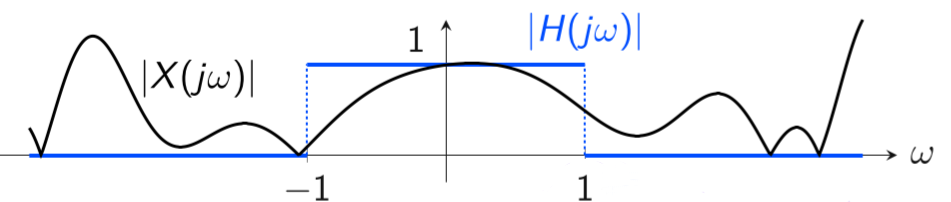
\includegraphics[width=8cm]{img/signalFreq.png}
\caption{Exemple de système LIT}
\end{figure}
Le fait de modifier le \textit{contenu fréquentiel} est appelé le \textbf{filtrage}.
\subsection{Type de filtre}
Il existe 3 grands types de filtres:
\begin{enumerate}
\item \textcolor{red}{Les filtres passe-bas}: ils vont atténuer et annuler les \textit{hautes-fréquences} pour ne laisser passer que les \textit{basses}.
\item \textcolor{red}{Les filtres passe-haut}: ils vont atténuer et annuler les \textit{basses fréquences} et ne laisser passer que les \textit{hautes}.
\item \textcolor{red}{Les filtres passe-bande}: ils ne vont laisser passer qu'une partie précise de fréquence. On peut voir cela comme la différence entre un filtre passe-bas d'envergure $A$ et un filtre passe-base d'envergure $B$ avec $A>B$. La différence $A-B$ est appelé la \textbf{largeur de bande}. 
\end{enumerate}
C'est grâce à cela que la radio fonctionne ou que les filtres photo fonctionnent.\\

\newpage % à enlever si écart 

\subsubsection{Les circuits RC}
Parmi les exemples typiques, on peut s'intéresser au circuit RC (cf: \href{https://github.com/Tfloow/Q4_EPL/blob/main/SyntheseCompilee/LELEC1370.pdf}{LELEC1370}). 
\begin{wrapfigure}{r}{.5\textwidth}
\centering
\includegraphics[width=5cm]{img/RC.png}
\caption{RC classique}
\end{wrapfigure}
En effet, on peut modéliser les équations d'un tel circuit comme suit:
\begin{align*}
x(t) &= R C \frac{du}{dt} + u(t) \longleftrightarrow\\
X(j \omega) = RC j \omega Y(j \omega) + Y(j \omega) &= Y(j \omega) (j\omega RC+1)\\
\frac{Y(j \omega)}{X(j \omega)} = H(j \omega) &= \frac{1}{1+ j \omega RC}\\
\text{Si } \omega_c = \frac{1}{RC}; |H(j\omega)| &= \frac{1}{\sqrt{1 + j(\omega / \omega_c)^2}}
\end{align*}
Ici, notre $\omega_c$ représente la \textcolor{blue}{fréquence de coupure}. C'est donc la valeur à partir de laquelle, on aura un changement notable de résultat.\\
Une chose à remarquer est que le déphasage lié à la fréquence angulaire augmente jusqu'à $\frac{\pi}{2}$. Peu perceptible au début, cela ne change rien fondamentalement.

\subsection{Filtres non-idéaux}
Un filtre parfait serait un filtre qui soit: nulle partout où on ne veut pas la fréquence et unitaire partout où on la veut.\\
\begin{wrapfigure}{r}{.5\textwidth}
\centering
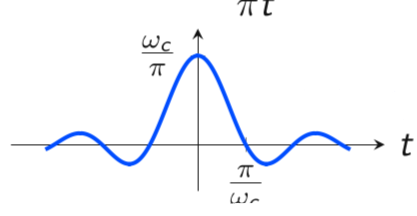
\includegraphics[width=6cm]{img/sinc.png}
\caption{Sinus cardinal}
\end{wrapfigure}
Mais comme vu au point \ref{window}, un tel signal en phasoriel correspond à:
\begin{align*}
H(j\omega) \longleftrightarrow h(t) = \frac{sin(\omega_c t)}{\pi t}
\end{align*}
Le gros soucis avec cela, c'est qu'on a une réponse actuelle du système qui dépend de quelque chose se passant dans le \textit{futur} donc pas vraiment physique. Le système n'est pas \textit{causal}.\\
On peut aussi noter qu'on aura un déphasage nul. En réalité, on cherche à avoir une déphasage linéaire car c'est simplement une modulation et est plus facilement corrigeable.

\subsubsection{Passe-bande non-idéal}
\begin{wrapfigure}{r}{.5\textwidth}
\centering
\includegraphics[width=6cm]{img/pbNonIde.png}
\end{wrapfigure}
Il en va de même pour le filtre passe-bande qui est composé de deux fonctions fenêtres comme suit:
\begin{align*}
|H(j\omega)| &= \sqcap \bigr(\frac{\omega + \omega_0}{B/2}\bigr) + \sqcap \bigr(\frac{\omega - \omega_0}{B/2}\bigr)\\
h(t) &= \frac{sin(Bt/2}{\pi t}2 cos(\omega_0 t)
\end{align*}
Comme au point précédent, c'est la non causalité et donc le manque de sens physique qui rend ce type de filtres idéaux impossibles.

\subsection{Filtre analogique}
Ce sont des filtres composés d'éléments \textcolor{blue}{passifs} et/ou \textcolor{blue}{actifs}. 
\begin{figure}[H]
\centering
\includegraphics[width=9cm]{img/analogique.png}
\caption{Réponse impulsionelle en fonction de la fréquence}
\label{analogique}
\end{figure}

Un filtre \textit{réel} a un $|H(j\omega)|$ qui ressemblent plus à la figure \ref{analogique}. Le \textbf{gabarit} précise les \textit{tolérances} qu'on accepte quand on design un filtre.
\begin{enumerate}
\item \textcolor{red}{Fluctuations bande passante}: on détermine un $\epsilon$ qui définit la largeur de bande passante.
\item \textcolor{red}{Zone de transition}: correspond au $\Delta$ qui indique la largeur de cette zone.
\item \textcolor{red}{Fluctuations bande bloquante}: la largeur de cette bande est définit via $\delta$.
\end{enumerate}

\subsubsection{Les filtres passe-bas}
\begin{center}
\begin{tabular}{|m{3cm}|m{5cm}|m{7cm}|}
\hline
\cellcolor[gray]{0.8} Nom &\cellcolor[gray]{0.8} Réponse impulsionnelle & \cellcolor[gray]{0.8} Avantages \& Inconvénients\\
\hline
Butterworth & $|H(j\omega)|^2 = \frac{1}{1+(\omega/\omega_c)^{2n}}$ & On a un filtre avec une \textit{fluctuation de bande passante} minime. Une \textit{zone de transition} plus ou moins élevé et une \textit{bande bloquante} qui tend vers 0.\\
\hline
Tchebychev Direct & $|H(j\omega)|^2 = \frac{1}{1+(\gamma T_n^2 (\omega /\omega_c)}$ &$\gamma$ est le \textcolor{blue}{facteur d'ondulation} et $T_n^2$ est une fonction oscillante à amplitude \textit{constante}(\textit{polynôme de Tchebychev de première espèce d'ordre $n$}). On a un filtre avec une \textit{fluctuation de bande passante} oscillante mais borné. Une \textit{zone de transition} rapide et une \textit{bande bloquante} qui tend vers 0 et plus vite que \textcolor{blue}{Butterworth}.\\
\hline
Tchebychev Inverse & $|H(j\omega)|^2 = \frac{\sqrt{\gamma}T_n(\omega_c/\omega}{1+(\gamma T_n^2 (\omega /\omega_c)}$ &$\gamma$ est le \textcolor{blue}{facteur d'ondulation} et $T_n^2$ est une fonction oscillante à amplitude \textit{constante}(\textit{polynôme de Tchebychev de première espèce d'ordre $n$}). On a un filtre avec une \textit{fluctuation de bande passante} plate. Une \textit{zone de transition} rapide et une \textit{bande bloquante} oscille de manière bornée (l'inverse de \textcolor{blue}{Tchebychev}).\\
\hline
Elliptiques/Cauer & $|H(j\omega)|^2 = \frac{1}{1+ \gamma R_n^2(\omega / \omega_n \zeta)}$ &$\gamma$ est le \textcolor{blue}{facteur d'ondulation}, $\zeta$ est le \textcolor{blue}{facteur de sélectivité} et $R_n^2$ est une fonction \textcolor{blue}{rationnelle elliptique}. On a donc un filtre où en modifiant les paramètres $\gamma$ et $\zeta$, on peut obtenir un filtre spécifique.\\
\hline
\end{tabular}
\end{center}

\subsubsection{Les filtres passe-haut}
\begin{center}
\begin{tabular}{|m{3cm}|m{5cm}|m{7cm}|}
\hline
\cellcolor[gray]{0.8} Nom &\cellcolor[gray]{0.8} Réponse impulsionnelle & \cellcolor[gray]{0.8} Avantages \& Inconvénients\\
\hline
Butterworth & $|H(j\omega)|^2 = \frac{1}{1+(\omega/\omega_c)^{2n}}$ & Est très similaire à son homologue passe-bas. Donc on a des bandes très plate et une zone de transition assez rapide dépendant de son degré.\\
\hline

\end{tabular}
\end{center}

\subsubsection{Les filtres passe-bande}
Pour obtenir un filtre passe-bande, on combine 2 filtres passe-bas. On doit réaliser le changement de variable suivant:
\begin{align*}
j\omega \rightarrow \frac{\omega_0^2 - \omega^2}{Bj\omega}
\end{align*}
Où $B$ est la largeur du filtre souhaitée et $\omega_0$ est la fréquence à laquelle on va centrer nos deux bandes (une \textit{positive} et \textit{négative}).

\subsubsection{Les filtres à encoche / notch}
Ce sont des filtres qui ne font passer qu'une seule fréquence \textit{spécifique}.
\begin{align}
H(j\omega) = \frac{(j\omega + j\omega_0)(j\omega - j\omega_0)}{(j \omega + \omega_0(cos(\theta) + j\sin(\theta))(j \omega + \omega_0(cos(\theta) -j\sin(\theta))) }
\end{align}

\subsubsection{Les filtres passe-tout}
Il existe également une famille de filtre qui fait \textit{tout passer}. Son utilité ? \textcolor{blue}{déphaser} de $+/- \pi$ un signal ce qui peut être fort utile !
\begin{equation}
H(j\omega) = \frac{(j\omega - 2)}{(j\omega + 2)}
\end{equation}


\section{Caractérisation d'un filtre} \label{Bode}
Pour se faire, on prend son équation de réponse impulsionnelle et on trace son diagramme de \textcolor{blue}{Bode}. (ne pas oublier que Bode c'est \textit{la norme} \textbf{et} \textit{l'argument})\\

Pour se faire, on utilise une échelle \textit{logarithmique}. On doit également \textcolor{blue}{factoriser} notre réponse impulsionnelle comme suit:
\begin{align}
|H(j\omega)| &= K \frac{|1 + \frac{j\omega}{\omega{z_1}}||\frac{j\omega}{\omega_{z_2}}|\bigr|(\frac{j\omega}{\omega_{z_3}})^2 + 2 \xi \frac{j\omega}{\omega_{z_3}}+1\bigr|}{|1 + \frac{j\omega}{\omega{p_1}}||\frac{j\omega}{\omega_{p_2}}|\bigr|(\frac{j\omega}{\omega_{p_3}})^2 + 2 \xi \frac{j\omega}{\omega_{p_3}}+1\bigr|}\\
20 &log(|H(j\omega)|)
\end{align}
Grâce aux propriétés des logarithmes, on peut séparer et additionner les multiplications et et divisions.\\
Ainsi, on trace morceau par morceau notre fonction et on va sommer ses différentes parties.
\begin{align*}
\textcolor{orange}{20 log|K|} + \textcolor{red}{20 log \bigr| \frac{j\omega}{\omega_{z_1}}\bigr|} + \textcolor{blue}{20 log(\bigr|1 + \frac{j\omega}{\omega_{z_2}}\bigr|)}
\end{align*}

\begin{figure}[H]
\centering
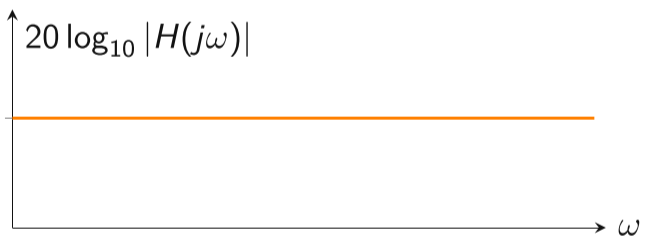
\includegraphics[width=4.5cm]{img/K.png}
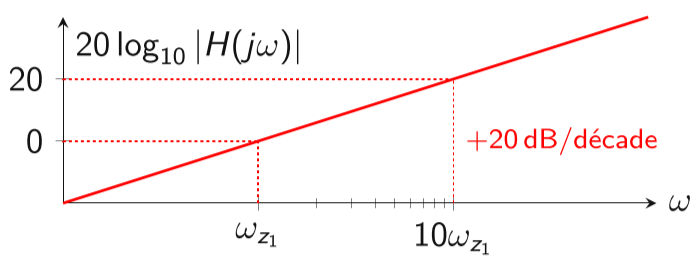
\includegraphics[width=5cm]{img/jomega.png}
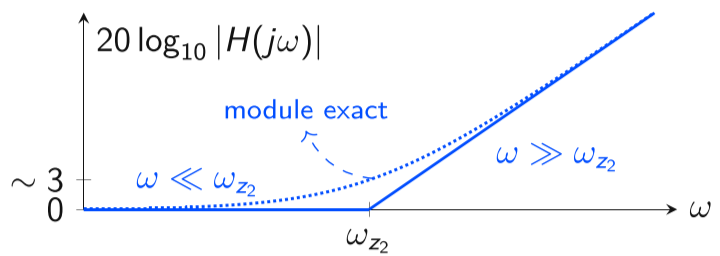
\includegraphics[width=5cm]{img/jomegacarre.png}
\end{figure}

et pour la version au \textit{carré} on a ceci. Il faut faire attention aux \textbf{asymptotes} qui peuvent se former !
\begin{align*}
\textcolor{green}{20log(\bigr|  \bigr(\frac{j\omega}{\omega_{z_3}}\bigr)^2 + 2 \xi \frac{j\omega}{\omega_{z_3}} +1 \bigr|)}
\end{align*}
\begin{figure}[H]
\centering
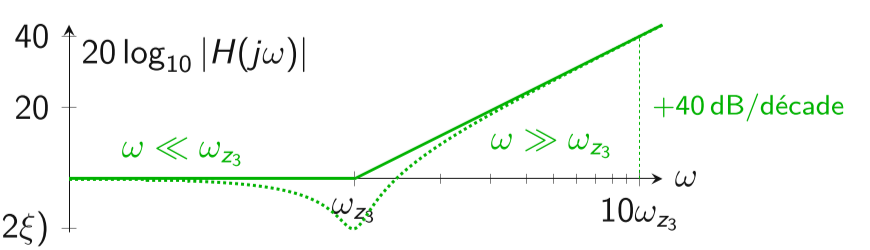
\includegraphics[width=6cm]{img/jomegamax.png}
\end{figure}
Après cela, on additionne/soustrait simplement nos courbes ensembles et on obtient notre \textit{première partie} du diagramme de \textcolor{blue}{Bode}.

\subsection{Argument}
Pour l'argument, le processus est le même si ce n'est qu'on ne met pas l'argument dans un logarithme mais est représenté sur une échelle logarithmique.\\
On trace nos différents arguments et on les somme.

\chapter{Transformée en Z}
\section{Transformée}
\subsection{Fonction de transfert}
La réponse $y$ à une entrée $u$ tel que $y = h \ast u $. Dans le domaine de $z$ on a $Y(z) = \mathcal{Z}\{h \ast u \} = H(z) U(z)$. Notre fonction de transfert est donc:
\begin{equation}
H(z) := \mathcal{Z}\{h\}
\end{equation}
Cela nous donne des informations sur la réponse \textit{impulsionnelle} et caractérise \textcolor{blue}{entièrement} le système LTI $\mathcal{H}$ (avec ROC).

\subsection{Semblant de vecteur propre}
Si on a un signal $z^n$ avec $|z| = \rho$, on peut établir les effets d'un système LTI sur ce signal:
\begin{align*}
\mathcal{H}\{z^n\} &= \sum_{k=-\infty}^{\infty} h[k]z^{n-k} = z^n \sum_{k=-\infty}^{\infty} h[k] z^{-k}\\
&= z^n \mathcal{Z}\{H(z)\} = z^n H(z)
\end{align*}
Donc $z^n$ est un \textbf{vecteur propre} de tout système LTI. $H(z)$ est un scalaire qui n'est autre qu'une valeur propre. $z^n \rightarrow H(z) z^n$.\par
Cela nous permet de traiter indépendamment un signal si celui est une \textit{combinaison linéaire} de $z^n$. (ex: $x[n] = X_1 z_1^n + X_2 z_2^n + X_3 z_3^n$)

\subsubsection{Valeur propre} 
Si $x$ est une combinaison linéaire de $z^k = \rho^k e^{i \omega k}$ on trouve les scalaires ainsi
\begin{align*}
\mathcal{H}\{x[k]\} &= \frac{1}{2 \pi} \int_{- \pi}^{\pi} X( \rho e^{i \omega}) \rho^k e^{i \omega k} d \omega\\
&= \frac{1}{2 \pi} \int_{- \pi}^{\pi} H(\rho e^{i \omega}) X(\rho e^{i \omega}) \rho^k e^{i \omega k} d\omega
\end{align*}
On peut remarquer que la \textbf{Transformée en Z} diagonalise le système linéaire.

\subsection{Passage depuis/vers autres représentations}
\begin{align*}
\sum_{k=0}^N a_k y[n-k] &= \sum_{k=0}^M b_k u[n-k]\\
\sum_{k=0}^N a_k \textbf{$z^{-k}$} Y &= \sum_{k=0}^M b_k \textbf{$z^{-k}$} U\\
Y &= \frac{\sum_{k=0}^M b_k \textbf{$z^{-k}$}}{\sum_{k=0}^N a_k \textbf{$z^{-k}$}} U
\end{align*}
On a les \textbf{zéros} de H comme étant les z pour lesquels $H = 0$ et les pôles de H sont les z pour lesquels $H \rightarrow \infty$.

\subsubsection{Représentation d'état}
\begin{align*}
x[n+1] &= Ax[n] + Bu[n]\\
y[n] &= Cx[n] + Du[n]\\
Y &= (C(zI - A)^{-1} B + D)U
\end{align*}
Le calcul de l'inverse montre que:
\begin{align*}
C(zI -A)^{-1} B & \text{ Fonction rationnelle avec } \frac{ordre \leqslant n-1}{ordre n}\\
C(zI -A)^{-1} B + D & \frac{ordre \leqslant n-1}{ordre n} + D = \frac{ordre n}{ordre n}
\end{align*}
Si un système admet une représentation d'état, alors $H(z)$ rationnelle. On a un \textit{dénominateur} qui est $det(zI - A)$ d'ordre n et un numérateur ordre $< n$ si pas de $D$, ordre $n$ sinon.\par
En général, si $H$ est rationnel et système est \textbf{causal}. L'ordre du dénominateur $\geqslant$ ordre numérateur et $h(0) \neq 0$.

\subsubsection{Passage}
Si on a:
\begin{align*}
Y &= HU = C(zI - A)^{-1} BU & H &= \frac{\sum_{k=0}^M b_k z^k}{\sum_{k=0}^{N} a_k z^k} \text{ avec } M \leqslant N\\
H &= \frac{z^{-N}}{z^{-N}}\frac{\sum_{k=0}^M b_k z^k}{\sum_{k=0}^{N} a_k z^k} & &= \frac{\sum_{k=0}^M b_k z^{k-N}}{\sum_{k=0}^{N} a_k z^{k-N}}
\end{align*}
On obtient ainsi l'équation:
\begin{equation}
\sum_{k=0}^N \tilde{a} y[n-k] = \sum_{k=0}^N \tilde{b}_k u[n-k]
\end{equation}

\subsection{Importance des pôles}
Si nous avons une fonction de \textit{transfert} $H(z) = q(z)/p(z)$ pour un système LTI.
\begin{align*}
Y(z) &= H(z) U(z) = \frac{q(z)}{p(z)} \frac{\tilde{q}(z)}{\tilde{p}(z)}\\
&= \frac{\Pi (z-b_i)}{\Pi (z-a_i)} \frac{\Pi (z- \tilde{b}_i)}{\Pi (z - \tilde{a}_i)}
\end{align*}
En réalisant une \textcolor{red}{décomposition simple}:
\begin{equation}
y[k] = \sum_i \gamma_i a_i^k + \sum_i \tilde{\gamma}_i \tilde{a}_i^k
\end{equation}
La partie à gauche est l'ensemble des \textcolor{blue}{pôles de la fonction de transfert} et à droite l'ensemble des \textcolor{red}{pôles de l'entrée}.\par
Notre réponse finale est une \textit{combinaison} d'exponentielles de taux:
\begin{itemize}
\item pôles de la fonction de transfert $a_i$
\item pôles de l'entrée $\tilde{a}_i$
\end{itemize}

\textcolor{red}{rajouter explication causalité après tp}


\chapter{Stabilité, Commandabilité \& Observabilité}

\textcolor{red}{Routh-Hurwitz ?}

En général, les systèmes réels sont causaux tel que $h[n] = 0$ pour $n<0$.
\section{Stabilité}
Il faut que: $\parallel h \parallel_1$ existe, que la \textbf{ROC} soit autour du cercle unité ou l'axe imaginaire, que les \textbf{pôles} soient dans le cercle unité ou à gauche du plan.
\subsection{BIBO}
Un système est \textbf{BIBO-stable} si pour toute entrée bornée, la sortie est bornée. Si un signal $x$ est borné  si $\exists B$ tel que $|x[k]| < B$ pour tout $k$. On note cela $\parallel x \parallel_{\infty} := sup_k |x[k]|$ \par 
Un système LTI de réponse impulsionnelle $h$ est BIBO-stable si et seulement si $\parallel h \parallel_1$ existe. $\parallel x \parallel_1 := \sum_k |x[k]|$ et $\parallel x \parallel_1 := \sum_{\tau = -\infty}^{\infty} |x[\tau]| d \tau$.
\begin{align*}
|y[n]| &= \left| \sum_{k \geqslant 0} u[n-k]h[k] \right| \leqslant \sum_{k \geqslant 0} |u[n-k]||h[k]| & & \text{ En utilisant l'inégalité triangulaire}\\
|y[n]| &= \parallel u \parallel_{\infty}  \sum_{k \geqslant 0} |h[k]| = \parallel h \parallel_1 \parallel u \parallel_{\infty} & & \text{ En supposant que notre signal d'entrée u est borné}\\
&\parallel y \parallel_{\infty} \leqslant \parallel h \parallel_1 \parallel u \parallel_{\infty} & & \blacksquare
\end{align*}
Cela est une nécessité sinon, notre système renvoie un signal qui diverge si sa fonction de transfert n'est pas bornée.

\subsubsection{Impact sur erreur de commande}
\begin{wrapfigure}{r}{.5\textwidth}
\centering
\begin{equation}
\mathcal{H}\{u\} = \mathcal{H} \{u_{nominal}\} + \mathcal{H}\{\Delta u\}
\end{equation}
\end{wrapfigure}
Si nous avons une entrée avec une erreur tel que $u = u_{nominal} + \Delta u$ et que $\parallel u \parallel_{\infty} \leqslant \epsilon$. Voir équation ci-contre.\par
L'erreur peut être borné par $\parallel h \parallel_1 \epsilon$ qui est un seuil qu'on impose.

\subsubsection{Vision fonction de transfert}
\begin{wrapfigure}{r}{.5\textwidth}
\centering
\begin{equation}
\sum_{k=0}^{\infty} |h[k] z^{-k}| \leqslant \sum_{k=0}^{\infty} |h[k]| = \parallel h \parallel_1
\end{equation}
\end{wrapfigure}
Si $h$ est causal et que $\parallel h \parallel_1$ existe, alors pour tout $z \notin B(0,1)$ on voit que:\par 
La convergence de $\mathcal{H}(z) = \sum_k h[k] z^{-k}$. On a un \textbf{ROC} qui contient $\mathcal{C}\setminus B(0,1)$ et tous les \textbf{pôles} sont dans $B(0,1)$.\par 
Si notre \textbf{ROC} est $\mathcal{C}\setminus B(0,r)$ pour $r< 1$ alors notre système est \textbf{BIBO-stable}. Si $\mathcal{H}$ est rationnelle et tous ses pôles sont dans $B(0,1)$ alors $h[n]$ est une somme d'exponentielle décroissante.

\subsubsection{Stabilité d'une fonction de transfert DT}
Système LTI en \textit{temps discret} de fonction de transfert $\mathcal{H}$
\begin{align}
\text{Bibo stabilité } &\Rightarrow \text{ ROC contient } \mathcal{C}\setminus B(0,1) &  \text{ ROC contient } \mathcal{C}\setminus B(0,r) \text{ pour } r<1 & \Rightarrow \text{ BIBO stabilité}
\end{align}

\subsubsection{Stabilité d'une fonction de transfert CT}
Système LTI en \textit{temps continu} de fonction de transfert $\mathcal{H}$. Si on est \textbf{BIBO-stable} les \textit{pôles} sont à \textbf{gauche} de l'axe imaginaire:
\begin{align}
&\text{BIBO stabilité } \Rightarrow \text{ ROC contient } \{x+iy: x \geqslant 0\} & &\text{ Roc contient } \{x + iy : x \geqslant - \epsilon\} \Rightarrow \text{ BIBO stabilité}
\end{align}

\subsection{Stabilité interne}
On veut qu'un système partant d'un point \textit{initial} ($u=0$) doit revenir à un équilibre ou ne pas diverger.\par
\underline{Définition:} Un équilibré $(x^{\ast},u^{\ast})$ \textbf{stable} si pour tout $\epsilon > 0$ il existe un $\delta > 0$ tel que $x(0) \in B(x^{\ast}, \delta) \Rightarrow x \in B(x^{\ast}, \epsilon)$ pour tout temps futur (si l'entrée reste $u^{\ast}$)\par 
\underline{Définition:} Un équilibré $(x^{\ast},u^{\ast})$ \textbf{attractif} si il existe un $\delta > 0$ tel que $x(0) \in B(x^{\ast}, \delta) \Rightarrow \lim_{t \rightarrow \infty} x(t) =  x_0$ (si l'entrée reste $u^{\ast}$) (\textit{asymptotiquement stable})\par 
Il ne faut pas confondre stabilité et attractivité car  stabilité est l'idée de ne pas diverger et attractif c'est l'idée de tendre vers un endroit.

\subsubsection{LTI}
Donc pour un système qui est du type $\frac{d}{dt}x(t) = Ax(t) + Bu(t)$ on va ramener l'équilibre à $(0,0)$ car plus simple (\textit{changement de variable si besoin}).\par 
Si $(x^{\ast}, u^{\ast})$ est un équilibre alors $0 = Ax^{\ast} + Bu^{\ast}$:
\begin{align*}
\Delta x &= x - x^{\ast} & \Delta y &= u - u^{\ast} & &\text{ Changement de variable}\\
\frac{d}{dt}(x^{\ast} + \Delta x) &= A(x^{\ast} + \Delta x) + (B(u^{\ast} + \Delta u) & \frac{d}{dt} \Delta x &= A \Delta x + B \Delta u & &\Delta x = 0, \Delta u= 0
\end{align*}

\subsubsection{temps continu}
Si on a $x(t) = v_1 e^{\lambda_1 t} +v_2 e^{\lambda_2 t} + ... + v_m e^{\lambda_m t} + v'_m t e^{\lambda_m t}$ Où on retrouve des multiplicités simples et multiples. \par 
\underline{Théorème:} Un système LTI en \textbf{temps discret} matrice $A$ et ses valeurs propres:
\begin{itemize}
\item $\mathbb{R}(\lambda_i) < 0$ pour tout i, alors \textbf{stable et attractif}
\item $\mathbb{R} (\lambda_i) > 0$ pour un i, alors \textbf{instable et non-attractif}
\item $\mathbb{R}(\lambda_i) \leqslant 0$ et $\mathbb{R}(\lambda_i)=0$ pour un i:
\begin{itemize}
\item Si multiplicité 1, alors \textbf{stable et non-attractif} 
\item Si multiplicité $>1$, alors \textbf{instable et non-attractif}.
\end{itemize}
\end{itemize}
On applique la même idée en \textcolor{red}{temps discret}.
\subsubsection{Oublie des conditions initiales LTI}
Si $x_0$ et entrée $u$ alors $x(t) = x_{libre}(t) + x_{forcée}(t)$. Le $x_{forcée}(t)$ dépend uniquement de $u$ comme si $x(0) = 0$.\par 
Si on a un système LTI attractif, $x_{libre} \rightarrow 0$ et une modification de $x_{forcée}$ a un petit impact sur la trajectoire.

\subsubsection{Non-linéaire}
En linéaire, un système est soit \textit{stable} ou \textit{instable} dans son ensemble. En \textbf{non}-linéaire, chaque équilibre est \textit{différent}.\par 
On peut linéariser autour d'un équilibre tel que $f(x^{\ast}, u^{\ast}) = 0$ ensuite on analyse graphiquement ou sur base de la linéarisation.\par
\underline{\textbf{Démarche :}} On linéarise autour d'un équilibre $(x^{\ast}, u^{\ast})$ tel que $f(x^{\ast}, u^{\ast}) =0$
\begin{align*}
f(x,u) &= \frac{\partial f}{\partial x} (x-x^{\ast}) +\frac{\partial f}{\partial u} (u - u^{\ast}) + O(...) & \frac{d}{dt} \tilde{x} &= A \tilde{x} + B \tilde{u} \text{ où } \tilde{x} = x - x^{\ast}
\end{align*}


\underline{\textbf{Exemple:}} $\dot{x} = f(x) = -x +x^3$ qui nous donne 3 équilibres $\{-1, 0, 1\}$. On peut voir \textit{graphiquement} que seul 0 est un équilibre attractif.
\begin{align*}
x = 0 &, f'(x) = -1 \text{ système linéarisé } \dot{\tilde{x}} = - \tilde{x} & x = 1 &, f'(x) = 2 \text{ système linéarisé } \dot{\tilde{x}} = 2 \tilde{x} 
\end{align*}

\subsection{Interne vs BIBO}
Avec une représentation d'état continu, la fonction de transfert est: $H(s) = C(sI - A)^{-1} B + D$ et:
\begin{align*}
&(sI-A)= & &\text{Diagonale } s-a_{ii} \text{ hors diagonale } -a_{ij}\\
&(sI-A)^{-1}= & & (\text{transposée des co-facteurs (déterminants de matrices }(n-1)\times (n-1))/ det(sI-A)
\end{align*}
Donc les pôles de la fonction de transfert $\mathcal{H}$ sont les valeurs propres de $A$. Via la stabilité des $vep$ de $A$ on peut savoir si les pôles sont stables.\par 
Stabilité interne $\Longrightarrow$ stabilité BIBO. Instabilité BIBO $\Longrightarrow$ instabilité interne stricte. Le contraire n'est pas vrai.\par

\section{Intermède algébrique} 
On peut remarquer que le polynôme caractéristique d'une matrice $A$ évalué en $A$ est la matrice \textcolor{red}{nulle}.
\subsection{Théorème de Cayley-Hamilton}
$p_A (A) = 0$ pour toute matrice \textit{carrée}. On sait que le $p_a$ se trouve via $det(xI - A)$. Si on évalue un polynôme à une matrice. \par 
On va transformer la matrice via $A^{k} = V \Lambda^k V^{-1}$ où $\Lambda$ est la matrice de ses valeurs propres.
\begin{align*}
p(A) &= \sum_{k=0}^n a_k A^k = \sum_{k=0}^n a_k V \Lambda^k V^{-1}
= V \left( \sum_{k=0}^n a_k \Lambda^k \right) V^{-1}\\
&= V \left(  \sum_{k=0}^n a_k \begin{pmatrix}
\lambda_1^k & & \\
 & \lambda_2^k & \\
& & \ddots
\end{pmatrix} \right) V^{-1} = V \begin{pmatrix}
p(\lambda_1) & & \\
 & p(\lambda_2) & \\
 & & \ddots
\end{pmatrix} V^{-1}
\end{align*}
Donc maintenant, si on remplace $p$ un polynôme quelconque par $p_a$ le polynôme caractéristique, on a des $p_a(\lambda_i)$. Le propre d'un valeur propre sur son polynôme propre est qu'il \textbf{annule} celui-ci. Donc notre matrice devient \textcolor{red}{nulle}.\par \noindent
\underline{Corollaire 1:} Si $A$ est $n \times n$, $A^n$ est une combinaison linéaire de $A^0, A^1, ... , A^{n-1}$.
\begin{align}
p_A (A) = 0 & \Leftrightarrow A^n + a_{n-1}A^{n-1} + ... + a_0 A^0 = 0\\
& \Leftrightarrow A^n = -a_{n-1} A^{n-1} - a_{n-2} A^{n-2} - ... - a_0 A^0 \label{eq:cor1}
\end{align}
\underline{Corollaire 2:} Si $A$ est $n \times n$ $A^{n+1}$ est une combinaison linéaire de $A^0, ..., A^{n-1}$. On reprend \ref{eq:cor1} et on multiple par A. \par  \noindent
\underline{Corollaire 3:} Si $A$ est $n \times n$ alors $A^k$ avec $k \geqslant n$ peut être exprimé en fonction de $A^0, ..., A^{n-1}$. (Ré-appliquer corollaire 2).

\section{Commandabilité}
\noindent 
\underline{Définition:} Un état $x^{\ast}$ est \textit{atteignable} si il peut être atteint au départ de 0 en un temps \textbf{fini}. C'est-à-dire que dans un temps T et une entrée $u$, $x[k+1] = Ax[k] + bu[k]$ et $x[0] = 0$. Au final $x[T] = x^{\ast}$.\par
L'espace d'atteignabilité est l'ensemble des états atteignables. On dit qu'un système est \textbf{commandable} si tout état est \textit{atteignable}.

\subsection{Analyse en temps discret}
On a un système de type $x[k+1] = A x[k] + bu[k]$ et $x[0] = 0$. Pour $x[1] = A 0 + bu[0] = bu[0]$, $x[2] = Ax[1] + bu[1] = Abu[0] +bu[1] = (Ab \quad b) \tilde{u}_{0 \rightarrow 1} $. Où $\tilde{u}_{0 \rightarrow 1} = \begin{pmatrix}
u[0]\\
u[1]
\end{pmatrix}
$. De manière générale:
\begin{equation}
x[T] = \begin{pmatrix}
A^{T-1} b & A^{T-2} b & \hdots & Ab & b
\end{pmatrix} \tilde{u}_{0 \rightarrow T-1}
\end{equation}
$x^{\ast}$ est atteignable en un temps T si il est dans l'espace des colonnes de $\begin{pmatrix}
A^{T-1} b & A^{T-2} b & \hdots & Ab & b
\end{pmatrix}$\par \noindent
\underline{Via corollaire 3:} pour $T \geqslant d-1$ alors on reste dans le même espace colonne.

\subsubsection{Matrice de commandabilité}
Soit un système $x[k+1] = Ax[k] + bu[k]$ où l'état $x$ est de dimension $d$, la matrice de \textcolor{red}{commandabilité} est:
\begin{equation}
\mathcal{C} := \begin{pmatrix}
A^{d-1} b & A^{d-2} b & \hdots & Ab & b
\end{pmatrix}
\end{equation}
\noindent \underline{Théorème:} l'état $x^{\ast}$ est atteignable ssi il est dans l'\textit{image} de $\mathcal{C}$ (son espace \textcolor{red}{colonnes}). L'espace d'\textit{atteignabilité} est l'espace \textit{colonnes} de $\mathcal{C}$.\par 
\noindent Le système est dit \textcolor{red}{commandables} si $\mathcal{C}$ est de \textbf{plein rang}. Donc l'espace \textit{colonne} est $\mathbb{R}^d$

\subsubsection{Commandabilité vs Controlabilité}
La \textbf{commandabilité}, on peut atteindre n'importe quel état depuis 0 en un temps \textit{fini}. \par 
La \textbf{controlabilité}, on peut atteindre 0 depuis n'importe quel état en un temps \textit{fini}

\subsection{Calculer $\mathcal{C}$}
On calcule $b$ et $Ab$ et après on itère pour avoir $A^k b = A(A^{k-1} b)$.\par \noindent
Si une matrice est de plein rang, son déterminant est non-nul. Pour des matrices \textbf{rectangulaires}, elle est de plein rang si elle a une \textit{sous}-matrice $d \times d$ de plein rang.

\section{Observabilité}
On peut distinguer les conditions initiales en se basant sur la trajectoire libre.\par \noindent
\underline{Définition:} un état/condition initiale $x_0 \neq 0$ n'est pas observable si il mène à une sortie $y$ identiquement nulle (pour tout temps) si l'entrée $u$ est nulle.\par \noindent
\underline{Définition:} un état/condition initiale $x_0 \neq 0$ est \textbf{non-observable} si il mène à une sortie $y$ identiquement nulle (pour tout temps) si l'entrée $u$ est nulle.\par \noindent
Donc un système est \textbf{observable} si il n'existe \textbf{aucun} état non-observable. L'espace \textbf{non-observable} est l'ensemble des $x_0$ non-observable.

\subsection{Analyse en temps discret}
Si on a des conditions initiales $x_0$ et qu'on se souvient de la corollaire 3 on a:
\begin{align*}
x[n] &= A^{n-1} x_0 & y[n] &= C A^{n-1} x_0
\end{align*}
\begin{wrapfigure}{r}{.5\textwidth}
\centering
\begin{equation}
\begin{pmatrix}
C\\
CA\\
CA^2\\
\vdots\\
CA^{n-1}
\end{pmatrix} x_0 = 0
\end{equation}
\end{wrapfigure}
Pour les $y[n] = 0$ pour tout $n$ et $x_0$ non observables si et seulement si l'équation ci-contre est respectée.\par 
Cette matrice s'appelle la matrice d'\textbf{observabilité} $\mathcal{O}$ et via la corollaire 3, on peut passer de $n-1$ à $d-1$.\par 
L'état $x_0$ est non-observable si $\mathcal{O}x_0 = 0$. L'espace des \textbf{états non observables} est $ker \{\mathcal{O}\}$. Si le système est entièrement observable, $\mathcal{O}$ est de plein rang.

\subsection{Exploitation de la linéarité}
Système observable $\rightarrow$ conditions initiales différentes mènent à réponses différentes.\par 
Système \textbf{pas} observable $\rightarrow$ si $\Delta x$ est dans l'espace non-observable, alors $x_0$ et $x_0 + \Delta$ mène à la \textcolor{red}{même} réponse.

\subsection{Résumé}
Observabilité: le fait de pouvoir distinguer la réponse \textcolor{red}{libre} de différentes conditions initiales. On se base sur la matrice d'\textbf{observabilité}.\par 
Cela ne dit pas si il est facile de \textit{retrouver} $x_0$ ni comment on le calcule en pratique. \textbf{Non-observable}: impossible de distinguer certains états, pas de solution si système existe \textit{déjà}. (on doit prendre en compte cela quand on design un système).

\chapter{Feedback}
\section{Introduction}
On veut pouvoir adapter les transformations du système en se basant sur les effets actuels.

\subsection{Solution naïve}
Si nous avons un équilibre en $x^*$ et $u^*$ tel que $0 = Ax^* + Bu^*$ et on y applique le changement de variable $\Delta x = x - x^*$ et $\Delta u = u - u^*$. En ayant un système attractif, $\lim_{t \rightarrow \infty} \Delta x (t) = 0$.\par
Dans le cadre d'un four à une équation $\dot{T} = Ku -\alpha (T-T_{ext})$ il faut que $u^* = a/K (T^* - T_{ext})$.\par 
Le problème est que notre système est \textbf{très susceptible} aux erreurs et peu efficace.

\subsubsection{L'inverse}
On pourrait être tenté d'inverser les effets d'un filtre pour pouvoir mieux appréhender le résultat $Y = GG^{-1}R = R$. Si on est en RC, la fonction serait $Cs + 1/R$ et $H = p/q$ avec $p$ et $q$ des polynômes:
\begin{equation}
deg(q) \geqslant deg(p) \text{ système non causal}
\end{equation}
Ce type e système est \textcolor{red}{impossible} en temps réel.\par 

\subsubsection{Erreur}
Si nous avons une petite erreur en entrée, ceci pourrait perdre son point d'équilibre et avoir des conséquences catastrophique. Ne pourrait marcher que dans des cas bien particuliers. 

\subsection{Solution par feedback}
\begin{figure}[H]
\centering
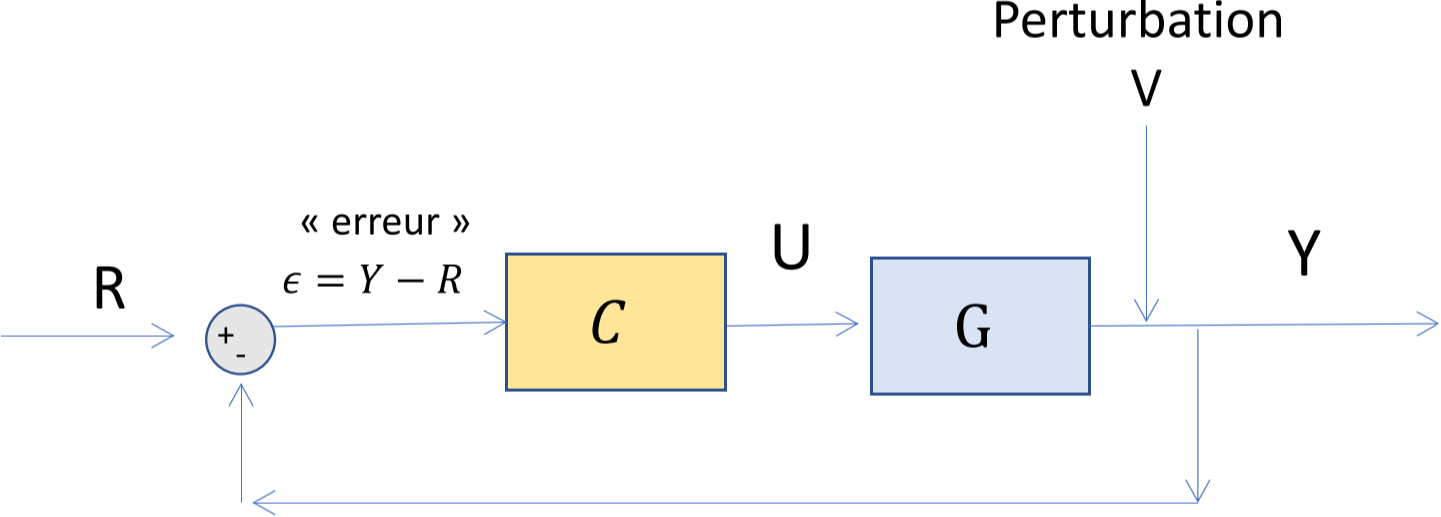
\includegraphics[width=7cm]{img/feedbeck.png}
\end{figure}
On va s'adapter à la sortie pour prendre en compte les erreurs qu'on pourrait avoir.
\begin{equation}
Y = \frac{CG}{1 + CG} R + \frac{1}{1 + CG}V
\end{equation}
On peut voir aussi comme $Y := TR + (1-T) V$ où $T \approx 1$ idéalement. Ceci n'est pas possible en général à toutes les fréquences. Donc on va souvent designer que $T \approx 1$ aux alentours de la solution en régime. Si $GC = \frac{p}{q}$
\begin{align*}
T &= \frac{\frac{p}{q}}{1+ \frac{p}{q}} = \frac{p}{q + p} & (1-T) &= \frac{q + p}{q + p} - \frac{p}{q + p} = \frac{q}{q + p}
\end{align*}

\subsection{Régulateur proportionnel}
Il faut bien régler le facteur $P$ dans l'équation $u = P(T_r -T)$. Si on prend une trop petite valeur, le système ne tend pas vers la solution idéale et trop élevé on consomme trop et converge rapidement. Souvent, l'idéal est $P = 1$.

\subsection{Régulateur proportionnel intégral}
Parfois, on peut faire face à des erreurs "\textit{statiques}". Ce sont des erreurs qui apparaissent quand la solution ne converge pas assez vite et semble converger vers la mauvaise valeur. On va donc ajouter un caractère \textbf{intégrateur} à l'équation pour qu'on force le système à se rapprocher du point de convergence.
\begin{equation}
u = P(T_r - T) + \int_{\tau  = 0}^{t} (T_r (t) - T(\tau)) d\tau
\end{equation}
Le problème est qu'on a souvent de l'overshoot et des oscillations qui peut s'avérer très ennuyant. On gagne en robustesse face à l'incertitude du modèle, à la variation des conditions et aux perturbations.

\subsubsection{Conclusions}
Si on a un système RC, on doit pas connaitre le R et C, fonctionne peu importe les paramètres. Si on connait, on peut \textbf{choisir} les pôles et le comportement.\par 
Cela stabilise si $k$ assez grand $(k>a)$. Si on connait $a$ on peut choisir les pôles.\par 
Cela est utilisé en industrie (surtout les modèles \textbf{PID} avec donc une dérivation). Fonctionne pas mal avec n'importe quel paramètre.

\subsection{Conclusions}
La régulation par \textbf{feedback} est plus \textit{robuste} et \textit{flexible} que la régulation en boucle \textbf{ouverte}. On peut commander ce système sans \textbf{aucune connaissance} plutôt correctement. On atténue les perturbations et on peut plus facilement stabiliser un système \textit{instable}.\par 
Il existe encore d'autres régulateurs. On peut bien adapter, de manière plus complexe, le comportement du système commandé. (choix des pôles, ...)


\end{document}
